\documentclass[11pt]{article}
\usepackage[utf8]{inputenc}
\usepackage[margin=1in]{geometry}
\usepackage{graphicx} % Required for inserting images
% \usepackage[draft]{graphicx} % Required for inserting images
\usepackage{enumitem}
\usepackage{comment}
\usepackage{amsmath}
\usepackage{amsfonts}
\usepackage{amsthm, amssymb}
\usepackage{thm-restate}
\usepackage{booktabs}
\usepackage[]{hyperref}
\hypersetup{
    colorlinks = true,
    linkcolor = blue,
    citecolor = blue
    }
    
\usepackage[
        noabbrev,
        capitalise,
        nameinlink,
    ]
    {cleveref}
\usepackage[dvipsnames]{xcolor}
\usepackage{bbm}
\usepackage{dirtytalk}
\usepackage{subcaption}
\usepackage{float}
\usepackage{tikz}
\usepackage{algorithm}
\usepackage[noend]{algpseudocode}
\usepackage{makecell}
\usetikzlibrary{arrows.meta,decorations.markings, calc, positioning}

\declaretheorem[name=Theorem,numberwithin=section]{thm}
\declaretheorem[name=Lemma,numberwithin=section]{lemma}
\declaretheorem[name=Assumption,numberwithin=section]{asmpt}
\declaretheorem[name=Proposition,numberwithin=section]{prop}
\declaretheorem[name=Corollary,numberwithin=section]{corollary}
\declaretheorem[name=Remark,numberwithin=section]{rmk}
\declaretheorem[name=Definition,numberwithin=section]{defn}
\newtheorem{claim}[theorem]{Claim}
\makeatletter
\renewcommand{\theHthm}{\thesection.\arabic{thm}}
\renewcommand{\theHlemma}{\thesection.\arabic{lemma}}
\renewcommand{\theHasmpt}{\thesection.\arabic{asmpt}}
\renewcommand{\theHprop}{\thesection.\arabic{prop}}
\renewcommand{\theHcorollary}{\thesection.\arabic{corollary}}
\renewcommand{\theHrmk}{\thesection.\arabic{rmk}}
\renewcommand{\theHdefn}{\thesection.\arabic{defn}}
\makeatother

\newcommand{\man}{M}
\DeclareMathOperator{\esssup}{esssup}
\definecolor{cyan}{cmyk}{1, 0.4, 0, 0} 
\newcommand{\ndfg}[1]{{\color{magenta}[Florian: #1]}}
\newcommand{\tls}[1]{{\color{cyan}[TLS: #1]}}
\newcommand{\pac}{\mathcal{P}_{2, \text{ac}}(\mathbb{R}^d)}
\newcommand{\posm}{\mathfrak{M}_+(\mathbb{R}^d)}
\newcommand{\HK}{\operatorname{HK}}
\newcommand{\PT}{\operatorname{PT}}


\usepackage[round]{natbib} 
\bibliographystyle{abbrvnat}

\title{On the Local Isometry of $(\mathfrak{M}_+(\Omega), \operatorname{HK})$ and $(\mathfrak{C}_\Omega, W_2)$}


\author{
\begin{tabular}{cccc} % Changed to 4 columns
% Row 1: 2 authors (2 columns each = 4 total)
\multicolumn{2}{c}{\makecell[c]{Tristan Luca Saidi\textsuperscript{\(\dagger\)}\\ \href{mailto:tsaidi@andrew.cmu.edu}{\nolinkurl{tsaidi@andrew.cmu.edu}}}} &
\multicolumn{2}{c}{\makecell[c]{Gonzalo Mena\textsuperscript{\(\dagger\)}\\ \href{mailto:gmena@andrew.cmu.edu}{\nolinkurl{gmena@andrew.cmu.edu}}}} \\[2em]
% Row 2: 2 authors (2 columns each = 4 total)
\multicolumn{2}{c}{\makecell[c]{Larry Wasserman\textsuperscript{\(\dagger, \ddagger\)}\\ \href{mailto:larry@stat.cmu.edu}{\nolinkurl{larry@stat.cmu.edu}}}} &
\multicolumn{2}{c}{\makecell[c]{Florian Gunsilius\textsuperscript{\(*\)}\\ \href{mailto:florian.felix.gunsilius@emory.edu}{\nolinkurl{fgunsil@emory.edu}}}} \\[1.5em]
\end{tabular}
\small\\ % Added a line break here to force affiliations down
\textsuperscript{\(\dagger\)}Department of Statistics and Data Science, Carnegie Mellon University\\
\textsuperscript{\(\ddagger\)}Machine Learning Department, Carnegie Mellon University\\
\textsuperscript{\(*\)}Department of Economics, Emory University
}


\begin{document}

\maketitle


\begin{abstract}
    The Hellinger-Kantorovich space provides a natural geometric setting for positive measures with varying total mass, with applications in areas such as statistics, machine learning, genomics, and imaging. Its differential-geometric properties are significantly less tractable than those of the Wasserstein space for probability measures, however. In this work we show that the classical representation of the Hellinger-Kantorovich geometry via Wasserstein geometry on the corresponding metric cone preserves some key differential-geometric structure. In particular, we provide an explicit procedure for obtaining a lifted Wasserstein geodesic for which the Hellinger-Kantorovich Riemannian geometry along the entire curve is preserved. This richer connection opens the door for computing many geometric quantities of interest using the tools developed for Wasserstein geometry. As an example, we show that this connection can be used to compute parallel transport on the Hellinger-Kantorovich space by lifting and applying existing tools from Wasserstein geometry, thereby circumventing the need for solving a high-dimensional parallel transport PDE arising from the covariant derivative. In the process of developing this Hellinger-Kantorovich parallel transport procedure, we also derive closed form expressions for the covariant derivative and the parallel transport operation on Euclidean metric cones. Finally, we provide simulations to illustrate the properties of parallel geodesics in the Hellinger-Kantorovich space.
\end{abstract}





\section{Introduction}


\section{Setup and Background}

In this section we describe the construction of Wasserstein space and its Riemannian structure.  We will then use this construction to define an analogous space corresponding to general positive measures instead of probability measures based on the principles of unbalanced transport. This construction follows closely the construction described in \cite{clancy2021interpolating, chewi2024statisticaloptimaltransport, liero2018optimal, liero2016optimal, chizat2018interpolating, kondratyev2016newoptimaltransportdistance}. 

We remark that our ultimate goal is to establish a stronger notion of equivalence between $(\mathfrak{M}_+(\Omega), \HK)$ and $(\mathcal{P}_2(\mathfrak{C}_\Omega), W_\mathfrak{C})$ (where $\Omega$ is a compact subset of $\mathbb{R}^d$). Therefore, in this section when discussing Wasserstein geometry $\mathcal{P}_2(\cdot)$, we will do so with $(\cdot) = \man$, a Riemannian manifold (potentially with boundary). However, when discussing Hellinger-Kantorovich geometry, we will only consider the space $\mathfrak{M}_+(\Omega).$ 

\subsection{Optimal Transport} Define $\mathcal{P}_{2}(\man)$ to be the set of probability measures with finite second moment over a complete, connected, boundaryless and $C^{\infty}$ Riemannian manifold $\man$ with metric tensor $g$. The $2$-Wasserstein distance between two probability measures $\mu, \nu \in \mathcal{P}_{2}(\man)$ is defined by
\begin{equation}
    W_2(\mu, \nu) = \inf_{\gamma \in \Gamma_{\mu, \nu}}\left(\int_{\man \times \man} d_M(x,y)^2\,\gamma(dx, dy)\right)^{1/2} \label{eq: 2 wasserstein dist}
\end{equation}
where $\Gamma_{\mu, \nu}$ denotes the set of couplings of $\mu$ and $\nu$. The $2$-Wasserstein distance (which we will henceforth refer to as the Wasserstein distance) is indeed a metric, which renders $(\mathcal{P}_{2}(\man), W_2)$ a metric space. A key result is that of Brenier, who showed that for $\man = \mathbb{R}^d$, the optimal coupling takes the form $(X, \nabla \varphi(X)), X \sim \mu$ for some convex $\varphi$ when $\mu$ is absolutely continuous with respect to the Lebesgue measure.

\begin{restatable}[Brenier]{thm}{} \label{brenier}
    Let $\mu, \nu \in \mathcal{P}_2(\mathbb{R}^d)$ be probability measures such that $\mu$ has a density, and let $X \sim \mu$. If $\gamma^*$ is optimal for \cref{eq: 2 wasserstein dist} with $\man = \mathbb{R}^d$, then there exists a convex function $\varphi:\mathbb{R}^d \rightarrow \mathbb{R}$ such that $(X, \nabla\varphi(X))\sim \gamma^*$. 
\end{restatable}

This theorem guarantees that if the source measure has a density, then the optimal transport coupling can be written as the source measure $\mu$ and $\nabla \varphi_\#\mu$, the pushforward of the source under some convex function -- note that the pushforward of a measure $\mu$ under a map $T$ is simply the measure $(T_\#\mu) (B) = \mu(T^{-1}(B))$ for all measurable $B$. The function $\nabla\varphi$ from \Cref{brenier} is often referred to as the \textit{Brenier map}. This key theorem of Brenier will be central to our construction of the Riemannian structure on the space of probability measures. We note that Brenier's theorem was later generalized to Riemannian manifolds, as described below. The result requires generalizing the notion of convexity and concavity to non-Euclidean settings. In particular, given a function $\psi: M \rightarrow \mathbb{R} \cup \{\pm \infty\}$ its \textit{infimal convolution} $\psi^c$ with a cost function $c$ is defined by 
\[\psi^c(y) = \inf_{x \in M}\left\{c(x,y) - \psi(x)\right\}.\]
We say $\psi$ is $c$-concave if and only if $\psi^{cc} = (\psi^c)^c = \psi.$

\begin{restatable}[Brenier-McCann, \citet{mccann2001polar}]{thm}{} \label{brenier-mcann}
    Let $(M, g)$ be a complete Riemannian manifold and let $\mu, \nu \in \mathcal{P}_2(\man)$ with $\mu \ll \operatorname{vol}_g$. Then there exists a $c$-concave function $\varphi: \man \rightarrow \mathbb{R}$ with $c(x,y) = d_M(x,y)^2$ such that the optimal plan (in the sense of \Cref{eq: 2 wasserstein dist}) is induced by a $\mu$-a.e. unique map
    \[T(x) = \exp_x\left(-\nabla\varphi(x)\right), \quad \gamma^* = (\operatorname{id}, T)_\# \mu\]
    where $\nabla$ is the Riemannian gradient and $\exp_p(v)$ is the Riemannian exponential map.
\end{restatable}

\subsection{Dynamic Formulation and Unbalanced Transport}

The optimal transport problem described above -- one which looks for an optimal coupling of source and target measures -- is often referred to as the \textit{static} formulation of optimal transport. An equivalent perspective comes from fluid mechanics, which arrives at the same metric structure through a different formulation. In particular, let $(v_t)_{t \geq 0}$ be a time dependent family of vector fields over $\man$, and consider the ODE $\dot X_t = v_t(X_t)$. Let $\mu_t$ denote the law of $X_t$, where $X_0 \sim \mu_0$ and $X_t$ evolves according to the ODE described previously. Then, the dynamics of $\mu_t$ obey the so-called \textit{continuity equation},
\begin{equation}
    \partial_t\mu_t + \operatorname{div}_g (\mu_t v_t) = 0 \label{eq: balanced continuity eqn}
\end{equation}
in the weak (or distributional) sense, where $\operatorname{div}_g$ is the Riemannian divergence. 
\begin{restatable}[Weak solutions to \Cref{eq: balanced continuity eqn}, \citet{santambrogio2015optimal}]{defn}{} \label{def: weak solutions}
    We say that a family of pairs $(\mu_t, v_t)$ solves the continuity equation on $(0, T)$ in the distributional sense if for any bounded and Lipschitz test function $\varphi \in C^1_c((0, T)\times \man)$ we have
    \[\int_0^T\int_{\man} \partial_t\varphi \, d\mu_tdt + \int_0^T\int_{\man} \langle\nabla\varphi,  v_t\rangle_g \, d\mu_tdt = 0.\]
\end{restatable}
It turns out, one can identify optimal transport maps with vector fields satisfying the continuity equation that are optimal in a certain sense. This gives rise to the \textit{dynamic} formulation of optimal transport.
\begin{restatable}[Benamou-Brenier, \citet{chewi2024statisticaloptimaltransport, ambrosio2012user}]{thm}{}
    Let $\mu_0, \mu_1 \in \mathcal{P}_{2}(\man)$ be absolutely continuous with respect to $\operatorname{vol}_g$. Then 
    \begin{equation*}
        W_2^2(\mu_0, \mu_1) = \inf \left\{\int_{0}^1\|v_t\|^2_{L^2(\mu_t)} dt \, \Bigg| \, (\mu_t, v_t)_{t \in [0,1]} \text{ satisfies \cref{def: weak solutions}}\right\}.
    \end{equation*}
    Moreover, if $M = \mathbb{R}^d$ then the optimal curve $(\mu_t)_{t\geq 0}$ is unique and is described by $X_t \sim \mu_t$, where $X_t = (1-t)X_0 + tX_1$ and $(X_0, X_1) \sim \gamma^* \in \Gamma_{\mu_0, \mu_1}$ with $\gamma^*$ being an optimal coupling.
\end{restatable}

In classical balanced transport, it is only possible to transport a measure $\mu$ to a measure $\nu$ if they have the same total measure. In many applications, it can be useful to consider situations where total mass can change over time. The dynamical formulation stated above, which considers minimum cost transport between probability measures, can be augmented to allow for \textit{unbalanced} transport. To do this, we use the \textit{continuity-reaction} equation, which allows for the creation and destruction of mass
\begin{equation}
    \partial_t\mu_t + \nabla \cdot (\mu_tv_t) = 4\beta_t\mu_t. \label{eq: unbalanced continuity eqn}
\end{equation}
This leads to an analogous notion of distance between general non-negative measures, commonly referred to as the \textit{Wasserstein-Fisher-Rao} (WFR) or the \textit{Hellinger-Kantorovich} (HK) distance. In fact, in \citet{liero2018optimal} it was shown that HK is indeed a metric on the space of non-negative measures over $\mathbb{R}^d$. 

\begin{restatable}[Hellinger-Kantorovich Distance, \cite{liero2018optimal, liero2016optimal, kondratyev2016newoptimaltransportdistance, chizat2018interpolating}]{defn}{}
    Let $\Omega\Subset \mathbb{R}^d$ and let $\mathfrak{M}_+(\Omega)$ denote the space of non-negative measures on $\Omega$. For any absolutely continuous $\mu_0, \mu_1 \in \mathfrak{M}_+(\Omega)$ we define the Hellinger-Kantorovich distance to be
    \begin{equation}
        \HK^2(\mu_0, \mu_1) = \inf\left\{\int_0^1 \left(\|v_t\|_{L^2(\mu_t)}^2 + 4|\beta_t|_{L^2(\mu_t)}^2\right)dt \, \Bigg| \, (\mu_t, v_t,  \beta_t)_{t\in [0,1]} \text{ solves \cref{eq: unbalanced continuity eqn}}\right\}.
    \end{equation}
\end{restatable}

\subsection{Riemannian Structure of Wasserstein and Hellinger-Kantorovich}

\noindent \textbf{The Tangent Space.} The dynamic formulations of balanced and unbalanced optimal transport are key ingredients in the Riemannian construction of $(\mathcal{P}_2(\man), W_2)$ and $(\mathfrak{M}_+(\Omega), \HK)$. In particular, we will construct the tangent space from space of solutions to the continuity equation. But seeing as there are an infinite number of solutions, (as adding a divergence free field does not change the marginal behavior of $\mu_t$) we need to establish a selection principle. To do so, we will define a notion of a \say{derivative} in a general metric space.

\begin{restatable}[Metric Derivative]{defn}{}
    Let $(\mathcal{X}, d)$ be a metric space and $(x_t)_{t \geq 0}$ be a curve in $\mathcal{X}$. The metric derivative of the curve at time $t$ is given by
    \begin{equation*}
        |\dot x|(t) \triangleq \lim_{s\rightarrow t}\frac{d(x_s, x_t)}{|s - t|}
    \end{equation*}
    provided that the limit exists. 
\end{restatable}

Now, for a pair of probability measures $\mu, \nu \in \mathcal{P}_{2}(\man)$ where $\mu$ admits a density, we will write $T_{\mu \rightarrow \nu}$ for the Brenier (or Brenier-McCann) map from $\mu$ to $\nu$ and we will write $|\dot \mu|$ for the metric derivative of a curve in $\mathcal{P}_{2}(\man)$ with respect to the Wasserstein metric.

\begin{restatable}[\citet{ambrosio2005gradient}]{thm}{}
    Let $(M, g)$ be a smooth and complete Riemannian manifold without boundary and let $(\mu_t)_{t\geq 0}$ be an absolutely continuous curve, i.e. $\mu_t$ admits a Riemannian density and $|\dot \mu_t|$ exists for all $t \geq 0$. Then for every family of vector fields $(v_t)_{t\geq 0}$ for which \cref{eq: balanced continuity eqn} holds, it holds that $|\dot \mu_t|(t) \leq \|v_t\|_{L^2(\mu_t)}$ for all $t \geq 0$. Moreover, there exists a unique family $(v_t)_{t\geq 0}$ such that \cref{eq: balanced continuity eqn} holds and for which $|\dot \mu_t|(t) = \|v_t\|_{L^2(\mu_t)}$ for every $t \geq 0$. This family is such that
    \begin{equation*}
        v_t = \lim_{h \rightarrow0^+}\left(h^{-1}\log_x(T_{\mu_t\rightarrow \mu_{t+h}}(x))\right) \qquad \text{ in $L^2(\mu_t)$}
    \end{equation*}
    and
    \begin{equation*}
        v_t = \min \left\{\|\tilde{v}_t\|_{L^2(\mu_t)}^2 \, \Big|\, \partial_t\mu_t + \operatorname{div}_g(\tilde v_t\mu_t) = 0\right\}
    \end{equation*}
    where $\log$ is the Riemannian logarithmic map. 
\end{restatable}

Note that result coupled with Brenier's theorem indicates that the velocity field that coincides (in an $L^2(\mu_t)$ sense) with the minimal norm solution and the metric derivative of the path is a limit of gradients. This key fact gives rise to the definition of the tangent space and the metric tensor for $(\mathcal{P}_{2}(\man), W_2)$ at a measure $\mu$. 

\begin{restatable}[Wasserstein Tangent Space, \citet{ambrosio2012user}]{defn}{}
    Let $\mu \in \mathcal{P}_2(\man)$. We define the tangent space to $\mathcal{P}_2(\man)$ at $\mu$ to be 
    \begin{equation}
        T_\mu \mathcal{P}_2(\man) = \overline{\left\{\nabla \varphi \, | \, \varphi \in C_c^{\infty}(\man)\right\}}^{L^2(\mu)}
    \end{equation}
    where $\overline{\{\cdot \}}^{L^2(\mu)}$ denotes the $L^2(\mu)$ closure and $C_c^{\infty}$ denotes the set of compactly supported and smooth maps. We also endow $T_\mu \mathcal{P}_2(\man)$ with the metric tensor
    \begin{equation}
        \langle \nabla \varphi_1, \nabla \varphi_2\rangle_{\mu} \triangleq \int_\man \langle\nabla\varphi_1, \nabla\varphi_2 \rangle_g \,d\mu 
    \end{equation}
    where $\langle \cdot, \cdot \rangle_g$ is the inner product defined by the metric tensor $g$.
\end{restatable}

We are now in a position to define analogous structure on the Hellinger Kantorovich space, $(\mathfrak{M}_+(\Omega), \HK)$. Starting from the augmented continuity equation, one can show that the minimum norm solution is unique and is the gradient of a potential. We can then use this to construct the tangent space and the metric tensor as we did for the Wasserstein space.
\begin{restatable}[\citet{clancy2021interpolating}]{prop}{}
    Let $\mu_t$ be an absolutely continuous measure in $\mathfrak{M}_+(\mathbb{R}^d).$ There exists a unique and minimal norm solution to the unbalanced continuity equation,
    \begin{equation*}
        (v_t, \beta_t) = \min\left\{\|\tilde v_t\|_{L^2(\mu_t)}^2 + 4|\tilde \beta_t|_{L^2(\mu_t)}^2  \, \Big| \, \partial_t\mu_t + \nabla \cdot (\tilde v_t \mu_t) = 4\tilde \beta_t \mu_t\right\}
    \end{equation*}
    with $(v_t, \beta_t) \in \overline{\left\{(\nabla \varphi, \varphi) \, | \, \varphi \in C^{\infty}_c(\mathbb{R}^d)\right\}}^{L^2(\mu_t) \times L^2(\mu_t)}$.
\end{restatable}

Now we can build out the tangent space analogy. Let $\Gamma \Subset U \Subset \Omega^\circ$ with $U$ open and define 
 \[\mathfrak{M}_+^\Gamma(\Omega) \triangleq\{\mu \in \mathfrak{M}_+(\Omega) : \operatorname{supp} \mu \subset \Gamma\}.\]
Although Clancy formulates the HK tangent and covariant derivative on $\mathfrak{M}_+(\mathbb{R}^d)$, while LMS \citep{liero2016optimal} work on ($\mathfrak{M}_+(\Omega)$, HK), the two descriptions coincide on any class of curves supported in a fixed interior region $\Gamma \Subset \Omega^\circ$. Accordingly, throughout this section we work on the localized class $\mathfrak{M}_+^\Gamma(\Omega)$ and use test potentials in $C^\infty_c(U)$ for a fixed open neighborhood $U$ of $\Gamma$ contained in $\Omega^\circ$.
 
\begin{restatable}[Hellinger-Kantorovich Tangent Space]{defn}{}
    For $\mu \in \mathfrak{M}_+^\Gamma(\Omega)$, we define the tangent space to be 
    \begin{equation}
        T_\mu \mathfrak{M}_+ = \overline{\left\{(\nabla \varphi, \varphi) \, | \, \varphi \in C_c^{\infty}(U)\right\}}^{L^2(\mu) \times L^2(\mu)}.
    \end{equation}
    We also endow $T_\mu \mathfrak{M}_+$ with the metric tensor
    \begin{equation}
        \langle s_1,  s_2\rangle_{\mu} \triangleq \int \langle\nabla\varphi_1, \nabla\varphi_2\rangle + 4\varphi_1\varphi_2 \,  d\mu
    \end{equation}
    for any $s_1, s_2\in T_\mu \mathfrak{M}_+$, with $s_i = (\nabla \varphi_i, \varphi_i)$ and $\varphi_i \in C_c^\infty(U)$. 
\end{restatable}

\noindent \textbf{The Covariant Derivative.} 
On an abstract manifold $(\man, g)$ that isn't embedded in an ambient space, we have no obvious way to compare vectors in the tangent space at two points $p, q \in \man$, $p \neq q$. Therefore, we need a way of connecting the separate vector spaces $T_p\man$ and $T_q\man$ when $p \neq q$. One can achieve this by defining a rule $\nabla$ for differentiating vector fields against each other on $\man$ in a way that preserves the structure of the metric $g$.

\begin{restatable}[The Covariant Derivative, \citet{petersen2006riemannian}]{defn}{}
    For a manifold $(\man, g)$ we define the covariant derivative $\nabla$ to be a rule that assigns to each pair of vector fields $X$, $Y$ over $\man$ another vector field $\nabla_XY$ satisfying 
    \begin{enumerate}
        \item \textit{Linearity:} $\nabla_{aX+bZ}Y = a\nabla_XY + b\nabla_ZY.$
        \item \textit{Leibniz/derivation property:} for $f \in C^{\infty}(\man)$ we have $\nabla_X(fY) = X(f)Y + f\nabla_XY$, where $X(f) = g(X, \nabla f)$ is the derivative of $f$ in the direction $X$.
    \end{enumerate}
\end{restatable}

While this gives us a way to connect tangent spaces, the covariant derivative might distort the geometry induced by the metric $g$ -- i.e. it might not be \say{metric compatible}. A fundamental result of Riemannian geometry, however, is that for any Riemannian manifold $(\man, g)$ there exists a \textit{unique} connection that is torsion free and is \say{metric compatible}. 

\begin{restatable}[The fundamental theorem of Riemannian Geometry, \cite{petersen2006riemannian}]{thm}{}
    If $\man$ is endowed with a Riemannian metric $g$, then there exists a unique connection $\nabla$ called the \textit{Levi-Civita connection} that is
    \begin{enumerate}
        \item \textit{Torsion free:} $\nabla_XY - \nabla_YX = [X,Y]$, where $[X,Y]$ is the Lie bracket of $X$ and $Y$. 
        \item \textit{Metric compatible:} $Xg(Y, Z) = g(\nabla_XY, Z) + g(Y, \nabla_XZ).$ 
    \end{enumerate}
\end{restatable}
In the case of $(\mathcal{P}_2(\mathbb{R}^d), W_2)$ and $(\posm, \HK)$ we can explicitly construct the covariant derivative, but one needs to manually verify that they are torsion free and metric compatible as neither spaces are finite-dimensional Riemannian Manifolds.


\begin{restatable}[Wasserstein Covariant Derivative, \citet{clancy2021interpolating, gigli2012second}]{prop}{} \label{Wasserstein covariant deriv}
    Let $\man$ be a $C^\infty$, complete and boundaryless manifold endowed with its Levi-Civita connection $\nabla^\man$. Let $(\mu_t)_{t\geq 0}$ be a curve through $\mathcal{P}_2(\man)$ with tangent field $\nabla \varphi_t$ solving \cref{eq: balanced continuity eqn}, and therefore driving the dynamics of $\mu_t$. Also let $v_t$ be another vector field along $\mu_t$ and let $\Pi_{\mu_t}$ be the orthogonal projection onto $T_{\mu_t}\mathcal{P}_2(\man)$ in $L^2(\mu_t)$. Then the differential operator $\nabla_{(\nabla\varphi_t)}^{W_2}$ given by
    \begin{equation*}
        \nabla_{(\nabla\varphi_t)}^{W_2}v_t = \Pi_{\mu_t}\left(\partial_t v_t + \nabla^{\man}_{( \nabla \varphi_t)} v_t \right)
    \end{equation*}
    is a valid covariant derivative, is torsion free, and is metric compatible.
\end{restatable}
This result establishes a closed form PDE describing a differential operator with the desired characteristics of the Levi-Civita connection. We also have an analogous covariant derivative for the Hellinger-Kantorovich space.

\begin{restatable}[Hellinger-Kantorovich Covariant Derivative, \citet{clancy2021interpolating}]{prop}{} \label{HK covariant deriv}
    Let $\Gamma \Subset U \Subset \Omega ^\circ$ with $U$ open and $\Omega \Subset \mathbb{R}^d$ and let $(\mu_t)_{t\geq 0}$ be a curve of measures supported on $\Gamma$ with tangent field $(\nabla \varphi_t, \varphi_t)$. Also let $(v_t, \beta_t)$ be another vector field along $\mu_t$ and let $\Pi_{\mu_t}$ be the orthogonal projection onto $T_{\mu_t}\mathfrak{M}_+$. Then the differential operator $\nabla_{(\nabla\varphi_t, \varphi_t)}^{\HK}$ given by
    \begin{equation*}
        \nabla_{(\nabla\varphi_t, \varphi_t)}^{\HK} \begin{pmatrix}
            v_t \\
            \beta_t
        \end{pmatrix} = \Pi_{\mu_t}\begin{pmatrix}
            \partial_t v_t + \nabla v_t \cdot \nabla \varphi_t + 2\beta_t\nabla\varphi_t \\
            \partial_t \beta_t + \frac{1}{2}\langle \nabla \beta_t, \nabla \varphi_t\rangle + 2\varphi_t\beta_t
        \end{pmatrix}
    \end{equation*}
    is a valid covariant derivative, is torsion free, and is metric compatible. 
\end{restatable}

\noindent \textbf{The Exponential and Logarithmic Maps.} For $\mathcal{P}_{2}(\man)$, the exponential map is defined to be $\mathbf{exp}_{\mu}(u) \triangleq (\exp(u))_\#\mu$ where $\exp(\cdot)$ is the exponential map of $\man$ and $u \in L^2(\mu)$. In the case of $\man = \mathbb{R}^d$, this operation is trivial -- we have
\begin{equation}\label{eq: wasserstein euclidean expmap}
    \mathbf{exp}_\mu(u) = (I_d + u)_\# \mu
\end{equation}
where $I_d$ is the identity map, $x \mapsto x$. In the case of the logarithmic map, things are analogous. We define $(\mathbf{log}_\mu\nu) (x) \triangleq \log_x(T_{\mu \rightarrow \nu}(x))$ where $T_{\mu \rightarrow \nu}$ is the Brenier map from $\mu$ to $\nu$. Note that we will denote $\overline{\log}$ as the normalized vector (with respect to the metric tensor). Again, in the Euclidean case this reduces to
\begin{equation}\label{eq: wasserstein euclidean logmap}
    (\mathbf{log}_\mu\nu )(x) = (T_{\mu \rightarrow \nu} - I_d)(x).
\end{equation}
In the case of Hellinger-Kantorovich, the exponential map and logarithmic maps are more challenging to describe and compute. When one assumes that $\mu_i \ll \pi_i$ where $\pi$ is the optimized coupling in \Cref{eq: let functional} (which means we are in the reaction-transport only regime), they admit a closed form as derived by \citet{cai2022linearized}. 

\begin{restatable}[Corollary of Proposition 4.8, \citet{cai2022linearized}]{prop}{} \label{HK exponential map closed form}
    Let $\mu_0, \mu_1 \in \mathfrak{M}_+(\Omega)$ and let $s_0 = (v_0, \beta_0)$ be a tangent field at $\mu_0$. Suppose further that for the optimal transport plan $\pi$ of the logarithmic entropy transport functional problem between $\mu_0$ and $\mu_1$, we have that $\mu_i \ll \pi_i$. Set $a_t = t\|v_0\|_2$, $b_t = 1 + t\beta_0/2$ and $S_t = \{x \in \Omega \, | \, (a_t(x), b_t(x)) = (0, 0) \}$, $q = \sqrt{a_t^2 + b_t^2}$ and $\varphi_t = \text{atan2}(a_t, b_t).$ Finally, let 
    \[T_t ( x) = x + \begin{cases}
        \frac{v_0(x)}{\|v_0(x)\|_2}\cdot \varphi_t(x) & \text{if } v_0(x) \neq 0 \\
        0 & \text{o.w.}
    \end{cases}.\]
    Then it holds that the curve given by $\mu_t = \mathbf{exp}_{\mu_0}(ts_0)$ where 
    \[\mathbf{exp}_{\mu_0}(ts_0) \triangleq (T_t)_\#(q_t(x)^2 \mu_0|_{\Omega \setminus S_t})\]
    is a unit speed HK geodesic between $\mu_0$ and $\mu_1$.  

\end{restatable}

\begin{restatable}[Proposition 4.1, \citet{cai2022linearized}]{prop}{} \label{HK logarithmic map closed form}
    Let $\mu_0, \mu_1 \in \mathfrak{M}_+(\Omega)$ and let $\pi = (\operatorname{id}, T)_\#\sigma$ be the minimizer in \Cref{eq: let functional} for some measurable $T: \Omega \rightarrow\Omega$ and $\sigma \in \mathfrak{M}_+(\Omega)$. Consider the Lebesgue decompositions of $\mu_0$ and $\mu_1$ with respect to the marginals of $\pi$, $\mu_0 = u_0 \sigma$ and $\mu_1 = u_1 (T)_\# \sigma$. Then 
        \[
        v_0(x) =
        \begin{cases}
        \dfrac{T(x)-x}{\|T(x)-x\|_2}\,
        \sqrt{\dfrac{u_{1}(T(x))}{u_0(x)}}\,
        \sin\bigl(\|T(x)-x\|_2\bigr),
        & T(x)\neq x,\\
        0, & T(x)=x,
        \end{cases}
    \]
    and
    \[
        \beta_0(x)
        =
        2\left(
        \sqrt{\dfrac{u_{1}(T(x))}{u_0(x)}}\,
        \cos\bigl(\|T(x)-x\|_2\bigr)-1
        \right).
    \]
    satisfy $\boldsymbol{\exp}_{\mu_0}(v_0, \beta_0) = \mu_1$.
\end{restatable}

These results indicate that we can compute the exponential and logarithmic map explicitly if we assume that the geodesic path of interest has no mass creation outside of the support of the initial measure -- intuitively, this means that all mass growth and destruction stems from the reaction component of the modified continuity equation. In many applications of interest, like genomics for example, this is a reasonable and an arguably desirable property.    

\section{Hellinger-Kantorovich Geometry via Cone Lifting} \label{sec: HK geometry via cone}

While Hellinger-Kantorovich geometry allows for a richer notion of transport, the tradeoff is that it induces more computational challenges. The tangent space, the covariant derivative and the exponential/logarithmic maps are all more challenging to describe and compute than their Wasserstein counterparts. Amazingly, \citet{liero2016optimal} show that Hellinger-Kantorovich geometry can be captured (in a delicate sense) from $W_2$ geometry on an augmented base domain. In particular, this construction entails lifting compactly supported positive measures from the base space $\Omega \Subset \mathbb{R}^d$ to probability measures on $\mathfrak{C}_{\Omega}$, the metric cone of the base space. Under a particular set of lifts, it turns out that the Wasserstein geometry on the cone recovers Hellinger-Kantorovich geometry on the original space.

\subsection{Metric Cones}

\begin{restatable}[Metric cone, \citet{burago2001course}]{defn}{} \label{def: metric cone}
    For a Riemannian manifold $(\man, g)$, the metric cone is
    \[\mathfrak{C}_\man = \man \times \mathbb{R}_{+} / (M \times \{0\})\]
    where a point in $\mathfrak{C}_\man$ is written as $(x, r)$. The metric tensor on the cone is given by $g_{(x,r)} = dr^2 + r^2g_x$, while the metric (as one would have in a metric space) is given by 
    \begin{equation*}
    d_{\mathfrak{C}}(z_0, z_1)^2 = r_0^2 + r_1^2 - 2r_0r_1\cos(d_{\man}(x_0, x_1) \land \pi)
    \end{equation*}
    for $z_i = (x_i, r_i)$.
\end{restatable} 

For metric cones of Euclidean space, we are fortunate in the sense that geodesics are available in closed form. This is made explicit and precise below.

\begin{restatable}[Geodesics on $\mathfrak{C}_{\Omega}$, $\Omega \Subset  \mathbb{R}^d$, \citet{liero2016optimal}]{prop}{}
    The function $Z(s; \cdot, \cdot ):\mathfrak{C}_\Omega \times \mathfrak{C}_\Omega \rightarrow \mathfrak{C}_\Omega$ given by 
    \begin{equation} \label{eq: cone geodesics}
        Z(s; z_0, z_1) = \left[X\left(s; z_0, z_1\right) , R\left(s; z_0, z_1\right)\right]
    \end{equation}
    where
    \begin{align*}
        R(s; z_0, z_1)^2 &= (1-s)^2r_0^2 + s^2r_1^2 + 2s(1-s)r_0r_1\cos(\min\{\pi, \|x_0 - x_1\|_2\}) \\
        \\[0.25ex]X(s; z_0, z_1) &= (1 - \rho(s; z_0, z_1))x_0 + \rho(s; z_0, z_1)x_1 \\
        \\[0.05ex]\rho(s; z_0, z_1) &= \begin{cases}
            \frac{1}{\|x_0 - x_1\|_2}\arccos\left(\frac{(1-s)r_0 + sr_1\cos(\|x_0 - x_1\|_2)}{R(s; z_0, z_1)}\right) & \text{for }\|x_0 - x_1\|_2 < \pi \\
            \frac{1}{2}\left(1 + \operatorname{sign}((1-s)r_0 + sr_1)\right) & \text{otherwise}
        \end{cases}
    \end{align*}
    is a unique constant-speed geodesic between $z_0$ and $z_1$ where $d_{\mathfrak{C}}(\gamma(s), \gamma(t)) = |t-s|d_{\mathfrak{C}}(z_0, z_1)$. 
\end{restatable}

From this closed form expression, we can directly compute the exponential and logarithmic map on $\mathfrak{C}_\Omega$, the proof for which we provide in \Cref{sec: proof of cone exponential and log map}.
\begin{restatable}[Exponential and Logarithmic maps on $\mathfrak{C}_\Omega$]{prop}{} \label{cone exponential and log map}
    Let $z_i = (x_i, r_i) \in \mathfrak{C}_{\Omega}$ and let $(v_x, v_r) \in T_{z_0}\mathfrak{C}_\Omega$ with $\|v_x\|_2 > 0$. Then for $0 < \|x_0 - x_1\|_2 < \pi$ we have
    \begin{equation} \label{eq: cone exp map}
        \exp^{\mathfrak{C}}_{z_0}((v_x, v_r)) = \left(x_1, r_1\right)
    \end{equation}
    with 
    \begin{equation*}
        x_1 = x_0 + \theta\frac{v_x}{\|v_x\|_2}, \quad r_1 = \sqrt{\|v_x\|_2^2r_0 + (v_r+r_0)^2}, \quad \theta = \operatorname{atan2}(r_0\|v_x\|_2, v_r + r_0)
    \end{equation*}
    and 
    \begin{equation} \label{eq: cone log map}
        \log_{z_0}^\mathfrak{C}(z_1) = \left[\frac{\sin(\|x_1 - x_0\|_2)r_1(x_1 - x_0)}{\|x_1 - x_0\|_2r_0}, r_1\cos(\|x_1 - x_0\|_2) - r_0\right].
    \end{equation}
\end{restatable} 

Finally, we provide a derivation of the covariant derivative and closed form parallel transport on $\mathfrak{C}_\Omega$ in \Cref{sec: cone parallel transport}. To obtain these objects we appeal to the theory of \textit{warped-product} manifolds \citep{o1983semi}, which are a class of product manifolds to which our cone space $\mathfrak{C}_\Omega$ belongs. 

\subsection{Lifting Measures, Geodesics and Tangent Vectors.}

We have established the structure of a metric cone, and now we have to map it back to our base space. Given a measure on $\mathfrak{C}_\Omega$, $\lambda \in \mathcal{P}_2(\mathfrak{C}_{\Omega})$ we can project it to a measure in $\mathfrak{M}_+(\Omega)$ with the map $\mathfrak{B}$ characterized by
\begin{equation} \label{eq: measure projection}
    \int_{\Omega} \phi(x)d\mathfrak{B}\lambda(x) = \int_{\mathfrak{C}_\Omega} r^2 \phi(x) d\lambda(x, r) \qquad \text{for all test functions }\phi \in C^0(\Omega).
\end{equation}
Note that, given a base measure $\mu$, there are infinitely many valid lifts of it to $\mathfrak{C}_\Omega$. \citet{liero2016optimal} show that one can replicate Hellinger-Kantorovich geometry on $\Omega$ through Wasserstein geometry on the cone space $\mathfrak{C}_\Omega$ by minimizing over all possible lifts. 

\begin{restatable}[Correspondence of $(\mathcal{P}(\mathfrak{C}_\Omega), W_2)$ and $(\mathfrak{M}_+(\Omega), \HK)$, \citet{liero2016optimal} Theorem 3.6]{thm}{} \label{HK cone variational prob}
    For any measures $\mu_0, \mu_1 \in \mathfrak{M}_+(\Omega)$ we have 
    \begin{equation} \label{eq: cone wasserstein and hk equivalence}
    \HK(\mu_0, \mu_1) = \min\left\{W_{\mathfrak{C}}(\lambda_0, \lambda_1) \,\Big|\, \lambda_i \in \mathcal{P}(\mathfrak{C}_\Omega),  \mathfrak{B}\lambda_0 = \mu_0, \mathfrak{B}\lambda_1 = \mu_1\right\}
\end{equation}
where $W_\mathfrak{C}$ is the 2-Wasserstein distance with respect to the cone metric $d_\mathfrak{C}.$
\end{restatable}
This incredible result allows us to leverage key aspects of Wasserstein geometry when analyzing and understanding the geometry of the unbalanced Hellinger-Kantorovich space. This connection will be a key aspect of our approach. But before describing how we will leverage this result, we need to address a significant challenge -- minimizing over all such lifts in \cref{eq: cone wasserstein and hk equivalence} is not computationally tractable. Fortunately, one can leverage \textit{another} equivalent formulation of the Hellinger-Kantorovich distance to obtain explicit lifts that are optimal in the sense of \cref{eq: cone wasserstein and hk equivalence}.
\\

\noindent \textbf{The Logarithmic Entropy Transport Functional.}
To compute the Hellinger-Kantorovich distance and a pair of optimal lifts, we will use an equivalent characterization. Let $\pi_j = \Pi^j_\#\pi$ be the marginals of the joint measure $\pi$ and define the Hellinger-Kantorovich entropy-transport functional as
\begin{equation} \label{eq: let functional}
    E(\pi; \mu_0, \mu_1) = \int_{\Omega}F\left(\frac{d\pi_0}{d\mu_0}\right)d\mu_0 + \int_{\Omega}F\left(\frac{d\pi_1}{d\mu_1}\right)d\mu_1 + \int_{\Omega \times \Omega}c(\|x_0 - x_1\|_2)d\pi
\end{equation}
where
\begin{equation*}
    c(L) = \begin{cases}
        -2\log(\cos(L)) & L < \pi/2 \\
        \infty & L \geq \pi/2
    \end{cases}
\end{equation*}
and $F(\rho) = \rho\log\rho - \rho + 1.$ \citet{liero2016optimal} show that 
\begin{align} \label{eq: let hk equivalence}
    \HK(\mu_0, \mu_1) &= \inf\left\{E(\pi;\mu_0, \mu_1)^{1/2} \, |\, \pi  \in \mathfrak{M}_+(\Omega \times \Omega), \pi_j  \ll \mu_j\right\}.
\end{align}
They also show that the logarithmic entropy transport functional gives us a way to compute optimal lifts in the sense of \cref{eq: cone wasserstein and hk equivalence}. In particular, assume that $\pi \in \mathfrak{M}_+(\Omega \times \Omega)$ is a minimizer of $E(\cdot\,; \mu_0, \mu_1)$ and for the marginals $\pi_i$ consider the Lebesgue decomposition $\mu_i = \sigma_i\pi_i + \mu_i^\perp$. Then the transport plan $\gamma_{\pi} \in \mathfrak{M}_+(\mathfrak{C}_{\Omega} \times \mathfrak{C}_{\Omega})$ defined by
\begin{multline}\label{eq: optimal lift}
    \gamma_{\pi}(dz_0, dz_1) = \delta_{\sqrt{\sigma_0(x_0)}}(dr_0)\delta_{\sqrt{\sigma_1(x_1)}}(dr_1)\pi(dx_0, dx_1) \\
    + \delta_1(dr_0)\mu_0^\perp(dx_0)\delta_{\mathfrak{o}}(dz_1) + \delta_1(dr_1)\mu_1^\perp(dx_1)\delta_{\mathfrak{o}}(dz_0) 
\end{multline}
and the associated lifts $\lambda_i = \Pi_{\#}^i\gamma_\pi$ are optimal for \cref{eq: cone wasserstein and hk equivalence}. This means we can solve the logarithmic-entropy-transport functional approach and use the optimal plan to construct appropriate lifts of the original measures onto the cone, described in detail in \Cref{alg: lift measures to cone}. This is important, as \Cref{eq: let hk equivalence} is implementable with standard unbalanced optimal transport solvers. 


\begin{algorithm}[H]
    \begin{algorithmic}[1] \label{alg: lift measures to cone}
        \caption{Lift measures from  $(\mathfrak{M}_+(\Omega), \HK)$ to $(\mathcal{P}_{2}(\mathfrak{C}_\Omega), W_2)$}
        \label{alg: let lift}
        \Require Measures $\mu_0, \mu_1 \in \mathfrak{M}_+(\Omega)$.  
        \State Solve logarithmic entropy transport functional minimization,
        \begin{align*} 
            \HK(\mu, \nu) &= \inf\left\{E(\pi;\mu, \nu)^{1/2} \, |\, \pi  \in \mathfrak{M}_+(\Omega \times \Omega), \,\Pi^1_{\#}\pi  \ll \mu, \, \Pi^2_{\#}\pi \ll \nu\right\}
        \end{align*}
        for $E$ defined in \cref{eq: let functional}, and let $\pi^*$ denote the optimal coupling for the problem above. 
        \State Compute the Lebesgue decompositions $\mu_i = \sigma_i\pi_i^* + \mu_i^\perp$.
        \State Lift $\mu_i$ to $\lambda_i$ via $\lambda_i = \Pi^i_{\#}\gamma_{\pi^*}$ with $\gamma_{\pi^*}$ defined in \cref{eq: optimal lift}.
        \State \Return $\lambda_0, \lambda_1  \in \mathcal{P}_{2}(\mathfrak{C}_{\Omega})$. 
    \end{algorithmic}
\end{algorithm}

\noindent \textbf{Geodesic Projections.} Note that these results indicate that optimal lifts are dependent on the source and target measures $\mu_0, \mu_1 \in \mathfrak{M}_+(\Omega)$ -- this indicates that we need to use caution when constructing algorithms on $\mathfrak{C}_\Omega$ to emulate Hellinger-Kantorovich geometry on $\Omega$. Fortunately, it holds that for a pair $\mu_0, \mu_1$, the $W_\mathfrak{C}$ geodesic between optimal lifts $\lambda_0, \lambda_1$ of $\mu_0, \mu_1$ projects back to a Hellinger-Kantorovich geodesic on $\Omega$. 

\begin{restatable}[\citet{liero2016optimal}, Corollary 4.4]{prop}{} \label{cone geodesics project to hk geodesics}
    For any optimal lift $\lambda_0, \lambda_1$ of $\mu_0, \mu_1$, an optimal plan $\gamma \in \mathcal{P}_2(\mathfrak{C}_\Omega \times \mathfrak{C}_\Omega)$ in the sense of $W_\mathfrak{C}$ induces a geodesic path in $(\mathfrak{M}_+(\Omega), \HK)$ connecting $\mu_0$ and $\mu_1$ given by
    \[\mu(s) = \mathfrak{B}\lambda(s) \qquad \text{with} \qquad \lambda(s) = Z(s; \cdot, \cdot)_\#\gamma\]
    where $Z(\cdot; z_0, z_1)$ is the geodesic interpolator described in \Cref{eq: cone geodesics}.
\end{restatable}
This result indicates that we can interpolate along a Hellinger-Kantorovich geodesic by lifting the source and target measures to $\mathfrak{C}_\Omega$, solving for the optimal plan, performing Wasserstein interpolation on $\mathfrak{C}_\Omega$, and projecting back via $\mathfrak{B}$. We provide a example of this interpolation procedure applied to two 

\begin{figure}[htbp] \label{fig:interpolation}
     \centering
     \begin{subfigure}{\textwidth}
         \centering
         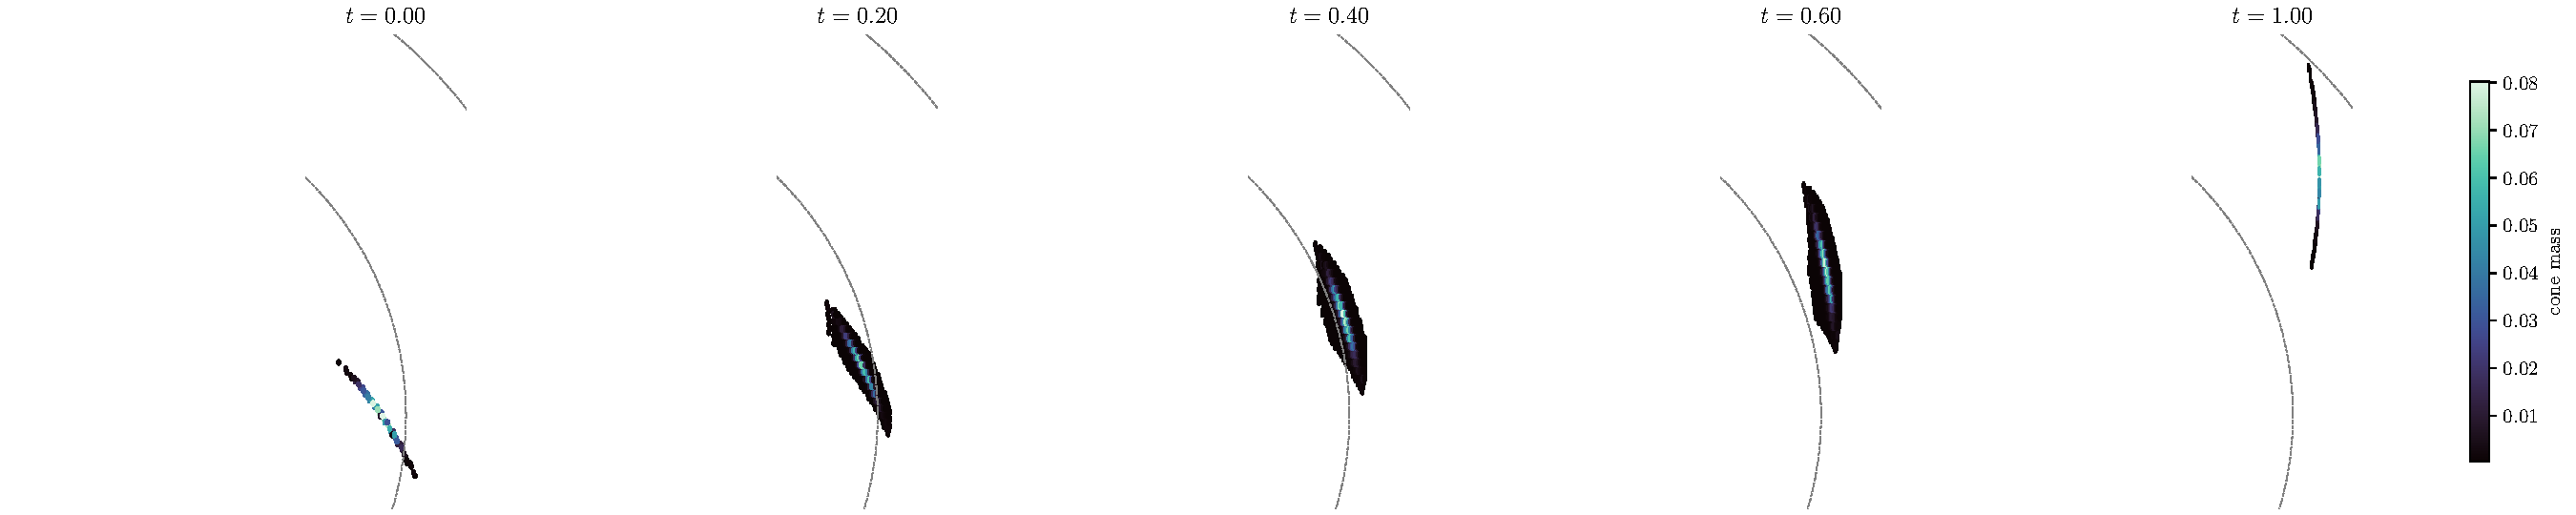
\includegraphics[width=\linewidth]{Figures/HK_cone_interpolation_polar.pdf}
         \caption{Wasserstein interpolation of $(\lambda_0, \lambda_1) = \operatorname{LETLift}(\mu_0, \mu_1)$ (\Cref{alg: let lift}) on $\mathfrak{C}_\Omega$  plotted in polar coordinates.}
     \end{subfigure}
     
     \vspace{1em} % Add vertical space between figures

     \begin{subfigure}{\textwidth}
         \centering
         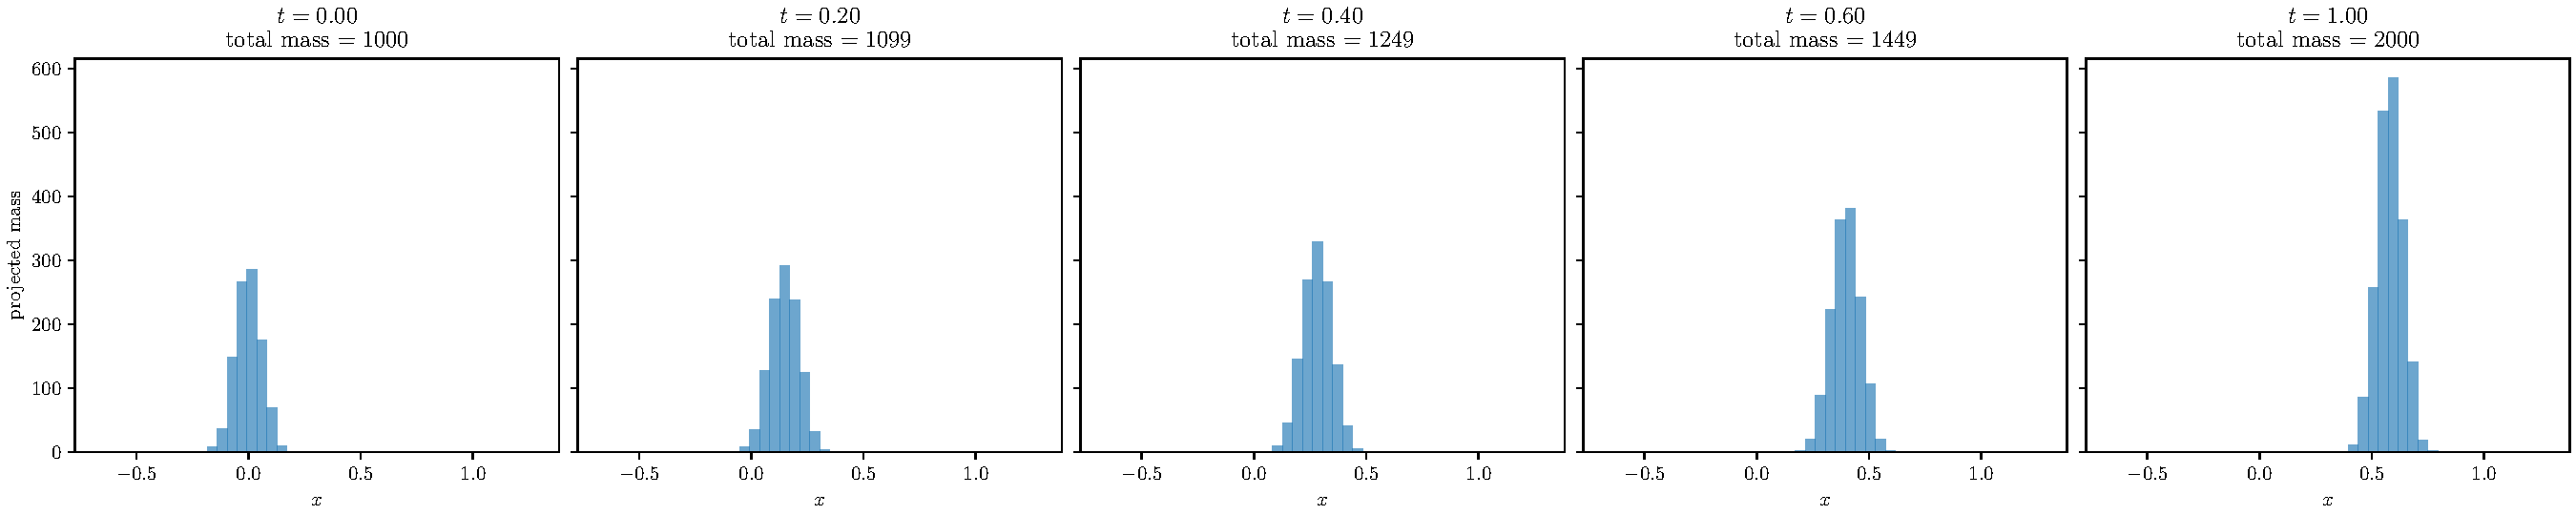
\includegraphics[width=\linewidth]{Figures/HK_cone_interpolation_projected.pdf}
         \caption{Hellinger-Kantorovich geodesic between $\mu_0, \mu_1$ obtained by projecting $\lambda_t$ from panel (a).}
     \end{subfigure}
     \caption{Visualization of Hellinger-Kantorovich interpolation using the lifting procedure described in \Cref{alg: let lift}. The measures $\mu_0, \mu_1$ consist of $n_0 = 1000$ and $n_1 = 2000$ draws from Gaussian probability measures with offset means. Note that we do \textit{not} normalize the empirical measures, and thus $\mu_0(\mathbb{R})\neq \mu_1(\mathbb{R})$.}
\end{figure}

\\
\noindent \textbf{Lifting Tangent Vector Fields.} Fortunately, lifting tangent vectors in a manner that is faithful to the dynamical formulation of Hellinger-Kantorovich geometry is tractable too. We'll define the vector field lifting operator as follows, 
\begin{align*}
    \mathcal{L}_{\mu, \lambda}: L^2(\mu; \mathbb{R}^d) \times L^2(\mu) \rightarrow L^2(\lambda; T\mathfrak{C}_\Omega) \quad \text{given by} \quad \mathcal{L}_{\mu, \lambda}[(v, \beta)](x,r) = (v(x), 2\beta(x)r)
\end{align*}
where $\mathfrak{B}\lambda = \mu$. For the rest of the paper, we may opt to drop the operator subscripts as they do not effect the functional form of the projection -- they merely denote the $L^2$ space in which the lifted objects live. 


\begin{restatable}[$\gamma_\pi$ Supported on a Map, \citet{clancy2022wasserstein}]{rmk}{} \label{clancy coupling supported on a map}
    Let $\pi$ be the optimal coupling from \Cref{alg: let lift}, suppose that $\mu_i^\perp = 0$, and suppose that $\mu_0, \mu_1$ are absolutely continuous with respect to Lebesgue. Then it holds that $\pi$ is supported on a map $T$ and the optimal coupling $\gamma_\pi$ of the optimal lifts $\lambda_0$ and $\lambda_1$ is supported on the assignment
    \[(x_0, r_0(x_0)) \mapsto (T(x_0), r_1(T(x_0))) \]
    implying that the radial conditional laws of $\lambda_0$ and $\lambda_1$ are deterministic. 
\end{restatable} 
\noindent With this in mind, we are now in position to define a complementary vector field \textit{projection} operator that takes cone Wasserstein tangent fields to HK tangent fields. Let $\lambda \in \mathcal{P}_2(\mathfrak{C}_\Omega)$ and let $u(x,r) = a(x,r) + b(x,r)\partial_r \in L^2(\lambda; \mathfrak{C}_\Omega)$ be vector field over the cone. We'll define the map  
\[\mathcal{P}_{\lambda}: L^2(\lambda; \mathfrak{C}_\Omega) \rightarrow L^2(\mathfrak{B}\lambda; \Omega) \times L^2(\mathfrak{B}\lambda) \]
as follows. Let 
\[v(x) = \frac{\int_{0}^\infty r^2a(x,r) \, d\lambda(r\,|\,x)}{\int_0^\infty r^2 \,d\lambda(r\,| \,x)} \quad \text{and} \quad \beta(x) = \frac{\int_0^\infty rb(x,r) \,d\lambda(r\, | \, x)}{2\int_0^\infty r^2 \,d\lambda(r\,| \,x)}\]
and define
\[\mathcal{P}_\lambda[u](x) = (v(x), \beta(x)).\]
With this definition in place, we are ready to present the following result relating the lifting operator $\mathcal{L}$ and the projection operator $\mathcal{P}.$
\begin{restatable}[Isometry of Lifting and Projection]{thm}{} \label{isometry}
    Let $\lambda \in \mathcal{P}_2(\mathfrak{C}_\Omega).$ Then
    \begin{enumerate}[label=(\alph*)]
        \item the lifting operator $\mathcal{L}_{\mathfrak{B}\lambda, \lambda}$ is an isometry between the Hilbert space $L^2(\mathfrak{B}\lambda; \Omega) \times L^2(\mathfrak{B}\lambda)$ equipped with the Hellinger-Kantorovich metric tensor and $L^2(\lambda; \mathfrak{C}_\Omega)$ equipped with the $\mathcal{P}_2(\mathfrak{C}_\Omega)$ metric tensor.
    \end{enumerate}  Moreover, if the radial law of $\lambda$ given $x$ is deterministic and not concentrated on $r = 0$, then 
    \[\mathcal{P}_\lambda[u](x) = \left(a(x, r(x)), \frac{b(x, r(x))}{2r(x)}\right)\]
    \begin{enumerate}[resume*]
        \item and the projection operator $\mathcal{P}_\lambda$ is the isometric inverse of $\mathcal{L}_{\mathfrak{B}\lambda, \lambda}$ $\lambda$ almost everywhere -- in particular, it is an isometry from $L^2(\lambda; \mathfrak{C}_\Omega)$ equipped with the $\mathcal{P}_2(\mathfrak{C}_\Omega)$ metric tensor and $L^2(\mathfrak{B}\lambda; \Omega) \times L^2(\mathfrak{B}\lambda)$ equipped with the Hellinger-Kantorovich metric tensor. 
    \end{enumerate}
\end{restatable}
We provide the proof of \Cref{isometry} in \Cref{sec: proof of isometry}. This result illustrates the following important fact: if we can construct lifts of geodesics where the conditional radial law of the measures are always \textit{deterministic}, then we have an explicit isometry between $T_{\mu_t}\mathfrak{M}_+$ and $T_{\lambda_t}\mathcal{P}_2(\mathfrak{C}_\Omega)$. In the next section we will describe a general lifting procedure that is optimal in the sense of \Cref{HK cone variational prob} \textit{and} satisfies this deterministic conditional radial law property.

\subsubsection{Method of Characteristics}

In this section we will characterize curves of measures by using the method of characteristics to solve for the Lagrangian paths and masses of individual particles. This will give us the foundation for producing cone lifts that have the deterministic conditional radial law property described above. \Cref{lifting by characteristics one} describes and proves the validity of a lifting procedure based on this principle. 

\begin{restatable}[Lifting by Characteristics]{prop}{} \label{lifting by characteristics one}
    Let $(\mu_t)_{t \in [0,1]}$ be a unique, absolutely continuous and constant speed geodesic in $\mathfrak{M}_+(\Omega)$, and suppose that there exist Borel fields $v_t: \Omega \rightarrow T\Omega$ and $\beta_t: \Omega \rightarrow \mathbb{R}$ solving the continuity-reaction equation,
    \[\partial_t \mu_t + \nabla \cdot(\mu_tv_t) = 4\beta_t \mu_t\]
    weakly. Assume that $v_t$ admits a Lagrangian flow $X_t$, i.e.
    \[\partial_t X_t(x) = v_t(X_t(x)), \quad X_0(x) = x\]
    and define,
    \[\eta_t \triangleq (X_t)_\# \mu_0, \quad r_t(X_t(x)) \triangleq \exp\left(2 \int_0^t \beta_s(X_s(x))\,ds\right).\]
    Then for any Borel $A \subset \Omega$
    \[\mu_t(A) = \int_A r_t^2 \, d\eta_t\]
    and $\lambda_t \triangleq (x \mapsto (x, r_t(x))_\#\eta_t$ is a valid lift of $\mu_t$, i.e. $\mu_t = \mathfrak{B}\lambda_t$. 
\end{restatable}
We provide the proof of \Cref{lifting by characteristics one} in \Cref{sec: proof of lifting by characteristics one}. The result indicates that we can obtain a valid lift of a curve of measures $\mu_t$ by integrating the reaction component $\beta_t$ along the particle-wise Lagrangian paths; this accumulated reaction will encode the radial coordinate of the location that a particle gets mapped to on the cone. Importantly, this lift satisfies the hypotheses of \Cref{isometry} part (b), which guarantee that the vector field projection and lifting operators are \textit{isometric inverses}. \Cref{lifting by characteristics two} formalizes this fact and proves that the proposed lifting procedure is indeed optimal in the sense of \Cref{HK cone variational prob}. 

Fortunately, in practice one does not need to approximate the integral to obtain the radial function $r_t$ along characteristics. Instead, one can simply leverage the following fact related to the logarithmic entropy transport functional problem -- we make this explicit in \Cref{radial update}. 

\begin{restatable}{prop}{} \label{radial update}
    The evolution of the radial coordinate $r_i$ in \Cref{alg:isometric-lift} satisfies 
    \[\frac{r_i(T_i(x))}{r_i(x)} = \sqrt{\frac{u_{i+1}(T_i(x))}{u_i(x)}}.\]
\end{restatable}
We provide a proof of \Cref{radial update} in \Cref{sec: proof of radial update}. With this fact, we can now provide an \textit{exact} algorithmic lifting procedure that avoids numerical integration. We provide the algorithm description in  \Cref{alg:isometric-lift}.

\begin{restatable}{rmk}{}
    As alluded to, the procedure for obtaining the lifted measures  and tangents described in \Cref{alg:isometric-lift} incurs no approximation error; in particular, $\lambda_i$, the characteristic values $X_i, r_i$ and the lifted tangents $V_i$ are all exact given population measures $\mu_0, \mu_1$. 
\end{restatable}


\begin{algorithm}[H]
\caption{Isometric lifting and interpolation procedure}
\label{alg:isometric-lift}
\begin{algorithmic}[1]
\Require Endpoints $\mu_0,\mu_1 \in \mathfrak{M}_+(\Omega)$, discretization level $N$.
\Ensure Discrete lifted path $(\lambda_i)_{i=0}^N$ on $\mathfrak{C}_{\Omega}$ and lifted tangent fields $(V_i)_{i=0}^{N-1}$.

\State Set $t_i=i/N$ for $i\in\{0,\dots,N\}$ and $\Delta t=1/N$.
\State Compute a discrete HK geodesic $(\mu_i)_{i=0}^N$ between $\mu_0$ and $\mu_1$ using \Cref{alg: let lift}.
\State Initialize $\eta_0 = \mu_0$ and $r_0(y)\equiv 1$.
\State Set $\lambda_0 = (y\mapsto (y,r_0(y)))_\# \eta_0$.

\For{$i=0$ to $N-1$}
    \State Solve the local HK / LET problem between $\mu_i$ and $\mu_{i+1}$.
    \State Let $\pi_i=(\mathrm{id},T_i)_\#\sigma_i$ be the induced Monge map and write
    $\mu_i=u_i\,\sigma_i$, $\mu_{i+1}=u_{i+1}\,(T_i)_\#\sigma_i.$
    \State Define the local HK logarithmic components
    \[
        v_i(y)=
        \begin{cases}
        \dfrac{1}{\Delta t}\dfrac{T_i(y)-y}{\|T_i(y)-y\|_2}\,
        \sqrt{\dfrac{u_{i+1}(T_i(y))}{u_i(y)}}\,
        \sin\bigl(\|T_i(y)-y\|_2\bigr),
        & T_i(y)\neq y,\\[2ex]
        0, & T_i(y)=y,
        \end{cases}
    \]
    \[
        \beta_i(y)
        =
        \frac{1}{2\Delta t}\left(
        \sqrt{\dfrac{u_{i+1}(T_i(y))}{u_i(y)}}\,
        \cos\bigl(\|T_i(y)-y\|_2\bigr)-1
        \right).
    \]
    \State Define the local radial multiplier (\Cref{radial update})
    \[
        q_i(y)= \sqrt{\frac{u_{i+1}(T_i(y))}{u_i(y)}}.
    \]
    \State Update the transported reference measure
    with $\eta_{i+1}= (T_i)_\#\eta_i.$
    \State Update the radial function on current positions by $r_{i+1}(z)= q_i(T_i^{-1}(z))\,r_i(T_i^{-1}(z)).$
    \State Set $\lambda_{i+1}= (z\mapsto (z,r_{i+1}(z)))_\#\eta_{i+1}.$
    \State Define the lifted tangent field $V_i= \mathcal{L}_{\mu_i,\lambda_i}(v_i,\beta_i).$
\EndFor

\State \Return $(\lambda_i)_{i=0}^N$ and $(V_i)_{i=0}^{N-1}$.
\end{algorithmic}
\end{algorithm}

\begin{figure}[htbp] \label{fig:isometric_interpolation}
     \centering
     \begin{subfigure}{\textwidth}
         \centering
         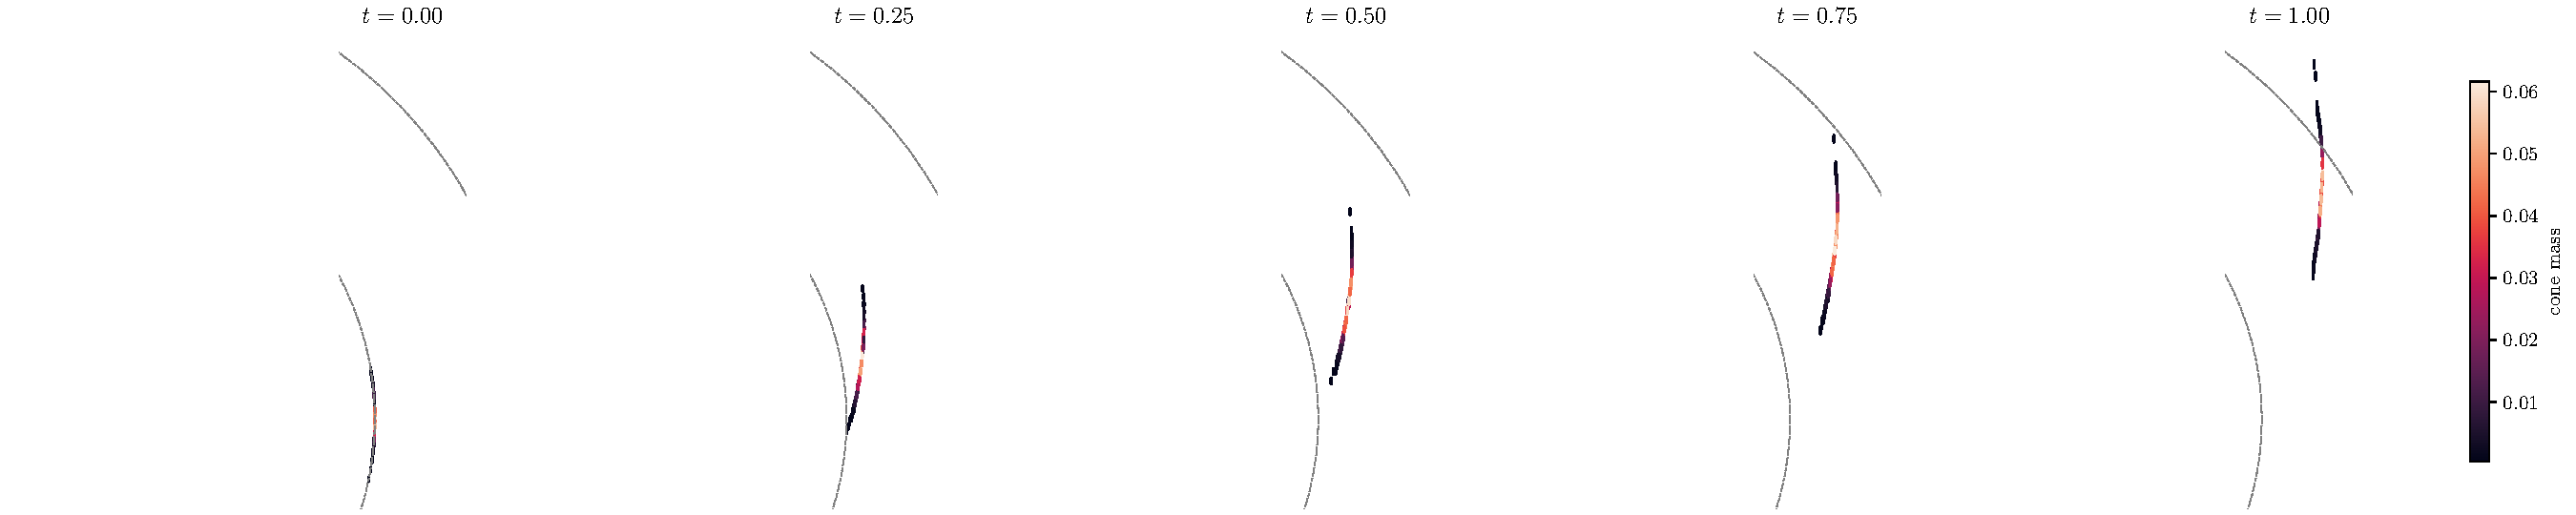
\includegraphics[width=\linewidth]{Figures/HK_cone_interpolation_recursive.pdf}
         \caption{Wasserstein interpolation of $(\lambda_0, \lambda_1) = \operatorname{IsometricLift}(\mu_0, \mu_1)$ (\Cref{alg:isometric-lift}) on $\mathfrak{C}_\Omega$  plotted in polar coordinates.}
     \end{subfigure}
     
     \vspace{1em} % Add vertical space between figures

     \begin{subfigure}{\textwidth}
         \centering
         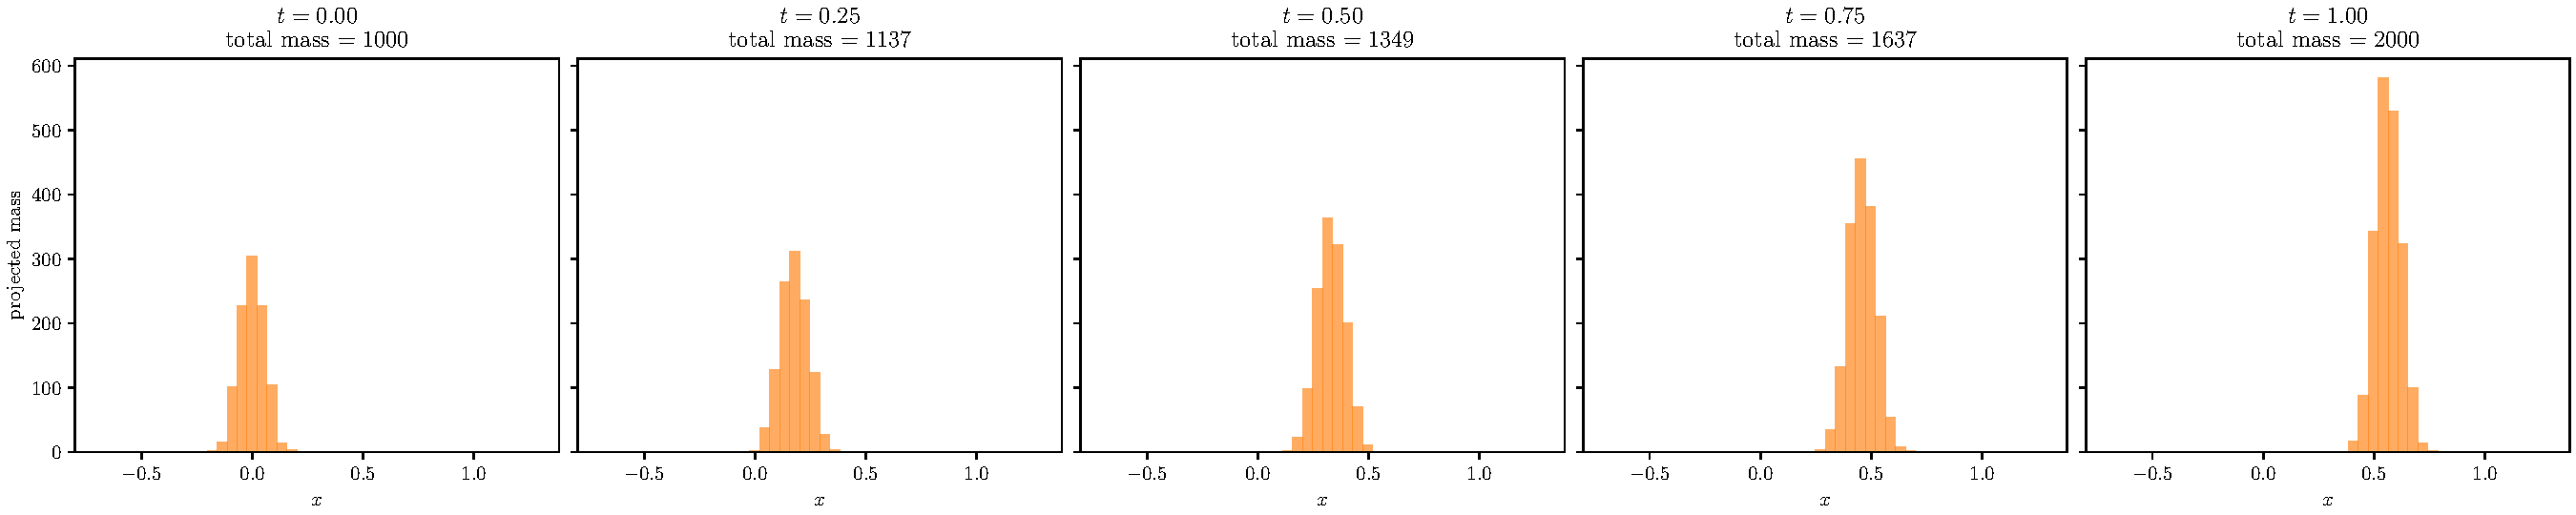
\includegraphics[width=\linewidth]{Figures/HK_cone_interpolation_recursive_projected.pdf}
         \caption{Hellinger-Kantorovich geodesic between $\mu_0, \mu_1$ obtained by projecting $\lambda_t$ from panel (a).}
     \end{subfigure}
     \caption{Visualization of Hellinger-Kantorovich interpolation using the lifting procedure described in \Cref{alg:isometric-lift} under the same settings as in \Cref{fig:cone_pt}. Observe that, unlike the LET lifted interpolant in \Cref{fig:cone_pt}, the conditional radial law of the measures $\lambda_t$ are deterministic for all $t$.}
\end{figure}

Now we will show that this lifting procedure is useful in a very powerful sense. In particular, as is clear from the construction, the lifted measures have the property that the conditional radial law is deterministic. As indicated by \Cref{isometry}, we know this ensures that the maps $\mathcal{P}_{\lambda_t}: T_{\lambda_t}\mathcal{P}_2(\mathfrak{C}_\Omega) \rightarrow T_{\mu_t}\mathfrak{M}_+$ and $\mathcal{L}_{\mu_t, \lambda_t}: T_{\mu_t}\mathfrak{M}_+ \rightarrow T_{\lambda_t}\mathcal{P}_2(\mathfrak{C}_\Omega)$ are isometric inverses. 


\begin{restatable}[Isometry and Optimality]{thm}{} \label{lifting by characteristics two}
    Suppose the assumptions and definitions of \Cref{lifting by characteristics one} hold, and further assume that $r_t(x)$ is nonzero for all $t$ and all $x$. Then the tangent lifting and projection maps \[\mathcal{L}_{\mu_t, \lambda_t}: L^2(\mu_t; \mathbb{R}^d) \times L^2(\mu) \rightarrow L^2(\lambda_t; T\mathfrak{C}_\Omega) \qquad \text{and} \qquad \mathcal{P}_{\lambda_t}: L^2(\lambda_t; T\mathfrak{C}_\Omega) \rightarrow L^2(\mu_t; \mathbb{R}^d) \times L^2(\mu_t)\] are isometric inverses. Moreover, the lifted tangent field $V_t \triangleq \mathcal{L}_{\mu_t, \lambda_t}(v_t, \beta_t)$ and the curve of measures $(\lambda_t)_{t \in [0,1]}$ satisfy the cone continuity equation, where $\lambda_t$ is both a $W_2$ geodesic on $\mathfrak{C}_\Omega$ and is an optimal lift, i.e.
    \[W_\mathfrak{C}(\lambda_0, \lambda_1) = \HK(\mu_0, \mu_1).\] 
\end{restatable}
We provide the proof of \Cref{lifting by characteristics two} in \Cref{sec: proof of lifting by characteristics two}. To the best of our knowledge, this result is the first to rigorously establish the existence and a explicit construction of an isometry of \textit{tangent spaces} between Hellinger-Kantorovich geodesics and lifted Wasserstein geodesics. As we shall see in later sections, this richer connection between the spaces enables the use of tools from Wasserstein geometry when solving for or computing Hellinger-Kantorovich objects. As an example, this connection will allow us to compute parallel transport on the Hellinger-Kantorovich space by computing Wasserstein parallel transport on the cone using the procedure described in \citet{saidi2026wassersteinparalleltransportpredicting} and projecting back. Before instantiating that example, we will demonstrate that the lifted geodesics inherit regularity properties directly from the Hellinger-Kantorovich interpolating geodesic. 


\subsection{Lifting Regularity}

In this section we will demonstrate that key regularity properties of the isometrically lifted procedure in \Cref{alg:isometric-lift} are inherited directly from standard assumptions on the HK geodesic $(\mu_t)$ on the base space. To the best of our knowledge, the same cannot be said for the lifted geodesic one obtains by taking the Wasserstein interpolation of the LET lifted endpoints in \Cref{alg: let lift}. This inheritance of regularity is key, as it ensures that many differential objects and operators exist for lifted geodesics. An example that we will explore is parallel transport, which only exists along sufficiently regular Wasserstein geodesics. 

\begin{restatable}[Admissible class]{asmpt}{} \label{admissible class}
    Let $\Gamma \Subset U \Subset  \Omega^\circ$ with $U$ open and $ \Omega\Subset \mathbb{R}^d$ where $\operatorname{diam}(\Omega)< \pi/2$. Also suppose that all measures are in the admissible class $\mathcal{C}\subset \mathfrak{M}_+^\Gamma(\Omega)$, where all pairs $\mu, \mu' \in \mathcal{C}$ 
    \begin{enumerate}[label=\textbf{(A.\arabic*)}, leftmargin=*, align=left]
        \item admit a minimizing LET coupling $\pi$ (\Cref{eq: let functional}) where $\mu^\perp = 0$, and thus $\pi$ is supported on a map $T$. 
        \item has a $\HK$ geodesic interpolant $\mu_t$ with a tangent velocity field $(v_t, \beta_t)$ satisfying \label{interpolant regularity}
        \begin{enumerate}
            \item uniform boundedness of $\beta_t:$  \[\operatorname{essinf}_{\mu_t} \beta_t \geq \beta_{\min} > -\infty \quad \text{and} \quad \esssup_{\mu_t}\beta_t \leq \beta_{\max} < \infty \quad \text{for all $t.$}\]
            \item uniform boundedness of $v_t:$  \[\sup_{t \in [0,1]} \|v_t\|_{L^\infty(\Gamma)} \leq M_v \quad \text{for some universal $M_v < \infty.$}\]
            \item square integrability:
            \[\int_0^1\|v_t\|_{L^2(\mu_t)}^2 \, dt < \infty \quad \text{and} \quad \int_0^1 |\beta_t|_{L^2(\mu_t)}^2 \, dt < \infty.\]
            \item spatial Lipschitzness:
            \[\sup_{t\in [0,1]}\operatorname{Lip}(v_t) \leq L_v \quad \text{and} \quad \sup_{t \in [0,1]}\operatorname{Lip}(\beta_t) \leq L_\beta \quad \text{for some universal $L_v, L_\beta <\infty.$}\]
        \end{enumerate}
    \end{enumerate}
\end{restatable}

The regularity described in \Cref{admissible class} is fairly standard, and we will show that it gives rise to lifted geodesics that have desirable properties. We start by showing that the boundedness of the reaction potentials $\beta_t$ guarantee that the lifted measures stay uniformly bounded away from the cone apex $\mathfrak{o}$. 

\begin{restatable}[Uniformly Bounded Lifts]{prop}{} \label{uniformly bounded lifts}
    The isometric lift of the geodesic interpolant $\mu_t$ of any $\mu_0, \mu_1 \in \mathcal{C}$ is uniformly bounded away from the cone apex $\mathfrak{o}$. In particular, for some $r_{\min}, r_{\max}$ independent of $t$ we have
    \[\operatorname{essinf}_{\mu_t} r_t \geq r_{\min} > 0 \quad \text{and} \quad \esssup_{\mu_t} r_t \leq r_{\max} < \infty \quad \text{for all $t$.}\]
    
\end{restatable}
We provide the proof of \Cref{uniformly bounded lifts} in \Cref{sec: proof of uniformly bounded lifts}. This property that the lifted measures stay uniformly bounded away from the cone apex ensures the existence of an open set on the cone where the metric is smooth and the set contains the supports of all lifted measures in the admissible class. This smoothness will be important for importing results from \citet{gigli2012second} regarding Wasserstein geometry on smooth Riemannian manifolds. 
We also have the following result, which guarantees that the lifted tangent velocity fields are spatially regular and integrable. 

\begin{restatable}[Uniformly Regular Lifts]{prop}{} \label{uniformly regular lifts}
    Let $\mu_0, \mu_1 \in \mathcal{C}$ admit a geodesic interpolant $\mu_t$ with tangent velocity $(v_t, \beta_t)$, and let $\lambda_t, V_t$ denote the isometrically lifted geodesic interpolant and its lifted velocity field. Then the lifted geodesic $\lambda_t$ is spatially regular in the sense that 
    \[  \int_0^1 \|V_t\|_{L^2(\lambda_t)}^2 \, dt < \infty  \quad \text{and} \quad\sup_{t\in[0,1]}\operatorname{Lip}_{\mathfrak{C}}(V_t) \leq L\]
    for some universal constant $L$.
\end{restatable}

The proof of \Cref{uniformly regular lifts} is provided in \Cref{sec: proof of uniformly regular lifts}. As with uniform boundedness, this uniform spatial regularity of the lifted geodesic tangents will enable us to import results from Gigli's second order analysis on the Wasserstein space. In particular, we will see that this regularity guarantees the existence of parallel transport. 




\section{Example: Hellinger-Kantorovich Parallel Transport}

As a concrete example of the richer connection between $(\mathfrak{M}_+(\Omega), \HK)$ and $(\mathfrak{C}_\Omega, W_2)$, we will use it to compute Hellinger-Kantorovich parallel transport; in particular, we will use recently developed tools for approximating \textit{Wasserstein} parallel transport, and then project back to the Hellinger-Kantorovich space. Since our lifting procedure yields an isometry of tangent spaces, the projected parallel transport coincides with the true Hellinger-Kantorovich parallel transport.  In the first part of this section we will describe the characterization of parallel transport via the covariant derivative. In the latter parts of this section, we will discuss the approximation scheme proposed by \citet{saidi2026wassersteinparalleltransportpredicting} and our proposed instantiation of it to compute Hellinger-Kantorovich parallel transport.   

\subsection{Exact Parallel Transport via the Covariant Derivative.} 
Intuitively, a vector field along a curve is \say{unchanging} loosely-speaking if its derivative is zero. Thus, in the context of abstract manifolds, a vector field along a curve is the parallel transport of a source vector if its covariant derivative along the curve is zero.
\begin{restatable}[\citet{lee2018introduction}]{defn}{} \label{parallel transport on general manifolds}
    Let $\man$ be a smooth Riemannian manifold. A smooth vector field $X$ along a smooth curve $\gamma$ is said to be parallel along $\gamma$ with respect to the Levi-Civita connection if $\nabla_{\dot \gamma}X \equiv 0$.
\end{restatable}
This characterization now allows us to define parallel transport on $(\mathcal{P}_2(\mathbb{R}^d), W_2)$ and $(\mathfrak{M}_+(\Omega), \HK)$ using the covariant derivative. Consider a smooth curve $\mu_t$ through $\mathcal{P}_2(\mathbb{R}^d)$ indexed by $t \in (0, 1)$ with the tangent field $\nabla \varphi_t$ driving its dynamics. 

\begin{restatable}[Wasserstein Parallel Transport PDE]{prop}{} \label{Wasserstein parallel transport pde}
    A vector field $v_t$ along $\mu_t$ is parallel along $\mu_t$ with respect to $\nabla_{(\nabla\varphi_t)}^{W_2}$ if
    \begin{equation*}
        \operatorname{div}_g \left(\mu_t\left(\partial_t v_t + \nabla v_t \cdot \nabla \varphi_t\right)\right) = 0 \qquad \text{for a.e. $t \in (0,1).$}
    \end{equation*}
\end{restatable}
\noindent \textit{Proof.} Due to \Cref{parallel transport on general manifolds} and \Cref{Wasserstein covariant deriv} we know that $v_t$ is a parallel vector field along the curve $\mu_t$ if $\Pi_{\mu_t}\left(\partial_tv_t + \nabla v_t \cdot \nabla\varphi_t\right) = 0$ for almost every $t \in (0,1).$ This is tantamount to the requirement that $\operatorname{div}_g\left(\mu_t(\partial_tv_t + \nabla v_t \cdot \nabla\varphi_t)\right) = 0$ since the $L^2(\mu_t)$ projection simply discards the divergence free portion of the vector field. \qed{}

The same approach is directly applicable for the Hellinger-Kantorovich case. Consider a smooth curve $\mu_t$ indexed by $t \in (0,1)$ with velocity field $(\nabla\varphi_t, \varphi_t)$. 

\begin{restatable}[Hellinger-Kantorovich Parallel Transport PDE]{prop}{} \label{HK parallel transport pde}
    A vector field $(v_t, \beta_t)$ along $\mu_t$ is parallel along $\mu_t$ with respect to $\nabla_{(\nabla\varphi_t, \varphi_t)}^{\HK}$ if
    \begin{align*}
        \nabla \cdot (\mu_t (\partial_tv_t + \nabla v_t \cdot \nabla \varphi_t + 2\varphi_t v_t + 2\beta_t \nabla\varphi_t)) = 0 
        \qquad \text{and} \qquad 
        \partial_t\beta_t + \frac{1}{2}\langle\nabla \beta_t, \nabla\varphi_t\rangle + 2\varphi_t \beta_t = 0.
    \end{align*}
\end{restatable}
\noindent \textit{Proof.} By \Cref{parallel transport on general manifolds} and \Cref{HK covariant deriv}, a vector field $(v_t, \beta_t)$ is parallel along $\mu_t$ if
\begin{align}
    \Pi_{\mu_t}\left(\begin{bmatrix}
        \partial_tv_t + \nabla v_t\cdot \nabla\varphi_t + 2\varphi_tv_t +  2\beta_t\nabla\varphi_t \\
        \partial_t\beta_t + \frac{1}{2}\langle\nabla \beta_t, \nabla\varphi_t\rangle + 2\varphi_t \beta_t
    \end{bmatrix}\right) = 0 \qquad \text{for a.e. $t \in (0,1).$ }
\end{align}
The orthogonal projection in the Hellinger-Kantorovich case is a Helmholtz decomposition of the vectorial portion of the argument (discarding the zero divergence component) and it leaves the mass creation term unchanged. Thus, we are left with the two conditions that we set out to prove. \qed{}

While \Cref{Wasserstein parallel transport pde} and \Cref{HK parallel transport pde} describe parallel transport along any curve, solving these PDEs in practice may be challenging, especially in high-dimensional settings. To this end, we will describe an alternative approximate approach for computing parallel transport along Hellinger-Kantorovich geodesics. To do this, we will lift the Hellinger-Kantorovich geodesic to the cone and use approximate Wasserstein parallel transport developed by \citet{saidi2026wassersteinparalleltransportpredicting}. The approach from this paper leverages the connection between parallel transport on a smooth, boundaryless and complete Riemannian manifold $\man$ and parallel transport on $\mathcal{P}_{2}(\man)$ -- a connection established by \citet{gigli2012second} -- to enable parallel transport on $\mathcal{P}_2(\man)$. 


\subsection{Approximate Hellinger-Kantorovich Parallel Transport}

As alluded to, we will demonstrate the utility of the isometric lifting procedure in \Cref{alg:isometric-lift} by using it to compute approximate Hellinger-Kantorovich parallel transport along geodesics. Our procedure, described in \Cref{alg: HK parallel transport}, combines the lifting procedure with approximate Wasserstein parallel transport. As we will show, the fact that the lifting procedure gives an explicit isometry of the Wasserstein and Hellinger-Kantorovich tangent spaces along the entire geodesic, this procedure is indeed valid. 

To formalize the setting, we need to ensure enough regularity on the lifted geodesic of measures for parallel transport to even exist. A sufficient condition is \textit{strong regularity}, defined in \Cref{strong regularity}. 

\begin{restatable}[Regular Curves, \citet{gigli2012second}]{defn}{} \label{strong regularity}
    Let $(\mu_t)_{t \in [0,1]}$ be an absolutely continuous curve of measures in $\mathcal{P}_2(\man)$ where $\man$ is a $C^\infty$, boundaryless, connected and complete manifold. We say that $(\mu_t)$ is strongly regular if its velocity vector field $(v_t)$ satisfies 
    \[\int_0^1\|v_t\|_{L^2(\mu_t)}^2\,dt < \infty \quad \text{and} \quad \sup_{t\in [0,1]}\operatorname{Lip}^\man(v_t) < \infty\]
    where $\operatorname{Lip}^\man(v_t)$ denotes the spatial Lipschitz constant of the field $v_t$. 
\end{restatable}

Fortunately, as we showed in \Cref{uniformly regular lifts}, the lifting procedure described in \Cref{alg:isometric-lift} yields a strongly regular geodesic when the endpoint measures $\mu_0$ and $\mu_1$ belong to the admissible class $\mathcal{C}$ defined in \Cref{admissible class}. One more detail to resolve, however, is the fact that the definition and results of \citet{gigli2012second} require $\man$ to be $C^\infty$, boundaryless, connected and complete. The domain $\mathfrak{C}_\Omega$ when restricted to radial coordinates in the range $[r_{\min}, r_{\max}]$ coming from \Cref{uniformly bounded lifts} is indeed a smooth and complete manifold, but it has a topological boundary. Fortunately, we can circumvent this through the following result.  

\begin{restatable}[Localized ambient setting for lifted geodesics]{thm}{} \label{cone ambient manifold}
Let $(\mu_t)_{t\in[0,1]}$ be an admissible HK geodesic and let $(\lambda_t,V_t)$ denote its deterministic isometric lift.
Then there exists an open manifold $\mathcal U$ and a complete smooth metric $\widetilde g_{\mathfrak C}$ on $\mathcal U$
such that:
\begin{enumerate}
    \item $\bigcup_{t\in[0,1]} \operatorname{supp}\lambda_t \Subset \mathcal U$.
    \item $\widetilde g_{\mathfrak C}$ agrees with the cone metric $g_{\mathfrak C}$ on a neighborhood of
    $\bigcup_t \operatorname{supp}\lambda_t$.
    \item the lifted curve $(\lambda_t)$ is a regular curve in $\mathcal P_2(\mathcal U,\widetilde g_{\mathfrak C})$, with velocity field $V_t$.
\end{enumerate}
Consequently, Gigli's parallel transport theory applies to $(\lambda_t)$, and the resulting objects depend only on the original cone geometry along the lifted curve.
\end{restatable}

We provide the proof of \Cref{cone ambient manifold} in \Cref{sec: proof of cone ambient manifold}. This result explicitly constructs a complete boundaryless Riemannian manifold with an interior compact subset whose geometry coincides exactly with that of the cone restricted to the support of all lifted measures in the admissible class. Thus, we will consider the geometry of $\mathcal{P}_2(\mathcal{U}, \tilde g_{\mathfrak{C}})$ in the following results to ensure compatibility with Gigli's theory. We now recall the following approximation result, which establishes that one can approximate $\mathcal{P}_2(\man)$ parallel transport by parallel transporting the tangent field along the Lagrangian paths on $\man$.

\begin{restatable}[\citet{gigli2012second}]{corollary}{} \label{approximation scheme}
    Let $(\man, g)$ be a smooth, complete and boundaryless Riemannian manifold, and suppose $
    \mu_0, \mu_1 \in  \mathcal{P}_{2}(\man)$ are probability measures that admit a strongly regular geodesic interpolant $\mu_t$ with a tangent velocity field $V_t$. For any $v \in T_{\mu_0}\mathcal{P}_2(\man)$ it holds that 
    \[\left\|\Pi_{\mu_t}(\PT^\man_{\mu_0 \rightarrow \mu_t}(v)) - {\PT}_{\mu_0 \rightarrow \mu_t}(v)\right\|_{L^2(\mu_t)} \leq  \left(e^{\int_0^1{\operatorname{Lip}}(V_s)\,ds} - 1\right)^2\|v\|_{L^2(\mu_0)}\left(\int_0^t{\operatorname{Lip}}(V_s)\,ds\right)^2\]
    where $\PT^\man_{\mu_0 \rightarrow \mu_t}(v)$ denotes the pointwise parallel transport (with respect to $\man$) of $v$ along the Lagrangian path defined by the $\mathcal{P}_2(\man)$ geodesic between $\mu_0$ and $\mu_1$. Moreover, the strong regularity of $\mu_t$ guarantees that $\Pi_{\mu_t}(\PT^\man_{\mu_0 \rightarrow \mu_t}(v))$ approximates ${\PT}_{\mu_0 \rightarrow \mu_t}(v)$, the Wasserstein parallel transport of $v$ along the geodesic $\mu_t$, in the sense that
    \[\left\|\Pi_{\mu_t}(\PT^\man_{\mu_0 \rightarrow \mu_t}(v)) - {\PT}_{\mu_0 \rightarrow \mu_t}(v)\right\|_{L^2(\mu_t)} \leq Ct^2 \quad \text{for some $C>0$ independent of $t$.}\]
\end{restatable}

\citet{saidi2026wassersteinparalleltransportpredicting} leverage this result to devise an approximation scheme that circumvents solving the parallel transport PDE. In particular, given an approximation resolution $N$, the approximate achieves an $O(N^{-1})$ error in an $L^2$ sense. 
\begin{restatable}[\citet{saidi2026wassersteinparalleltransportpredicting}]{corollary}{} \label{approximation scheme full geodesic}
    Let $v \in T_{\mu_0}\mathcal{P}_2(\man)$, let $N \in \mathbb{N}$, define $s = 1/N$ and define the maps
    \[\widehat \PT_k \triangleq \Pi_{\mu_t}(\PT^\man_{\mu_{(k-1)s} \rightarrow \mu_{ks}}(v)) \quad \text{for $k \in \{1, \dots, N\}$}.\]
    Then we have the following approximation bound,
    \[\left\|\left(\widehat \PT_N \circ \cdots \circ \widehat \PT_1\right)(v) - \PT_{\mu_0 \rightarrow \mu_1}(v)\right\|_{L^2(\mu_1)} = O(N^{-1}).\]
\end{restatable}
Thus, one can circumvent solving the Wasserstein parallel transport PDE in \Cref{Wasserstein parallel transport pde} through this approach, which instead requires computation of parallel transport on $\man$. This is typically much easier, as it usually amounts to solving an ODE -- in some cases, including ours, parallel transport is available in closed form. With this Wasserstein parallel transport approximation result, it seems natural to compute Hellinger-Kantorovich parallel transport by lifting to $\mathfrak{C}_\Omega$ and doing Wasserstein parallel transport there. The validity of this idea is formalized below in \Cref{commutator}.

\begin{restatable}[Lifted and projected parallel transport commute]{thm}{} \label{commutator}
    Let $(\mu_t)_{t\in[0,1]}$ be an admissible HK geodesic and let $(\lambda_t)_{t\in[0,1]}$
    denote its deterministic isometric lift. Fix $0 \le s < t \le 1$. Then for every
    $u \in T_{\lambda_s}\mathcal{P}_2(\mathcal U)$ it holds that
    \[
    \Big(\PT^{\mathrm{HK}}_{\mu_s \rightarrow \mu_t}
    \circ \mathcal{P}_{\lambda_s}\Big)(u)
    =
    \Big(\mathcal{P}_{\lambda_t}\circ
    \PT^{\mathfrak C}_{\lambda_s \rightarrow \lambda_t}\Big)(u).
    \]
    In particular, if $u=\mathcal{L}_{\mu_s,\lambda_s}[\mathbf u_s]$ for some
    $\mathbf u_s\in T_{\mu_s}^{\mathrm{HK}}$, then
    \[
    \mathcal{P}_{\lambda_t}\!\left[\PT^{\mathfrak C}_{\lambda_s \rightarrow \lambda_t}(u)\right]
    =
    \PT^{\mathrm{HK}}_{\mu_s \rightarrow \mu_t}(\mathbf u_s).
    \]
\end{restatable}
\begin{proof}
    This result follows trivially from the fact that $\mathcal{L}, \mathcal{P}$ are isometric inverses (\Cref{lifting by characteristics two}) and parallel transport commutes with isometries \citep{gallier2013isometries}.
\end{proof}

This result indicates that the lifting procedure of \Cref{alg:isometric-lift} allows Hellinger-Kantorovich to inherit the parallel transport approximation result from Wasserstein. We explicitly write out the entire procedure in \Cref{alg: HK parallel transport} and we describe the approximation error bound in \Cref{parallel transport approx entire geodesic}. 

\begin{algorithm}[H]
\caption{Approximate HK parallel transport via cone transport}
\label{alg: HK parallel transport}
\begin{algorithmic}[1]
\Require Endpoints $\mu_0, \mu_1 \in \mathfrak{M}_+^\Gamma(\Omega)$, source tangent
$\mathbf u_0 \in T_{\mu_0}\mathfrak{M}_+$, approximation resolution $N$.
\Ensure Approximation
$\widehat{\mathbf u}_{1,N}$ of
$\PT^{\mathrm{HK}}_{\mu_0\rightarrow\mu_1}(\mathbf u_0)$.
\State Set $s = \frac{1}{N}$ and $
t_k = ks$ for $k=0,\dots, N.$
\State Compute lifts $\left((\lambda_i)_{i = 0}^N, (V_i)_{i = 0}^N\right) = \operatorname{IsometricLift}(\mu_0, \mu_1, N)$ via \Cref{alg:isometric-lift}.
\State Lift the source tangent:
\[
U_{0} = \mathcal{L}_{\mu_0,\lambda_0}[\mathbf u_0]
\in T_{\lambda_0}\mathcal P_2(\mathcal U).
\]

\For{$k=1$ to $N$}
    \State Let $T_k:\mathcal U\to\mathcal U$ denote the optimal Monge map sending
    $\lambda_{t_{k-1}}$ to $\lambda_{t_k}$.
    \State Form local approximation described in \Cref{approximation scheme},
    \[ U_{k} = \Pi_{\lambda_t}\left((x,r) \mapsto \PT^\mathfrak{C}_{(x,r) \rightarrow T_k(x,r)}\left( U_{k-1}\right) \right)\]
    \hspace{\algorithmicindent} using cone parallel transport (see \Cref{sec: cone parallel transport}). 
\EndFor

\State Map back to the HK tangent space with $\widehat{\mathbf u}_{1, N}
=
\mathcal{P}_{\lambda_1}\big(U_{N}\big).$

\State \Return $\widehat{\mathbf u}_{1, N}$.
\end{algorithmic}
\end{algorithm}

\begin{restatable}[Approximation of HK parallel transport by cone transport]{thm}{} \label{parallel transport approx entire geodesic}
    Let $(\mu_t)_{t\in[0,1]}$ be an admissible HK geodesic and let
    $(\lambda_t,V_t)$ denote its deterministic isometric lift. Let $\mathbf u_0 \in T_{\mu_0}\mathfrak{M}_+$ and let
    $\widehat{\mathbf u}_{1, N}$ be the output of
    \Cref{alg: HK parallel transport} with input $\mathbf u_0$. Then
    \[
    \left\|
    \widehat{\mathbf u}_{1, N}
    -
    \PT^{\mathrm{HK}}_{\mu_0\rightarrow\mu_1}(\mathbf u_0)
    \right\|_{L^2(\mu_1)}
    = O(N^{-1}).
    \]
\end{restatable}

\begin{proof}
    By \Cref{approximation scheme full geodesic}, we know that 
    \[\left\|U_N  - \PT_{\mu_0  \rightarrow \mu_1}^{W_\mathfrak{C}}(U_0)\right\|_{L^2(\lambda_N)} = O(N^{-1}).\]
    Applying \Cref{commutator} completes the proof.
\end{proof}

We remark that the procedure requires one to compute parallel transport on the cone space $\mathfrak{C}_\Omega$. In \Cref{sec: cone parallel transport} we derive the covariant derivative on $\mathfrak{C}_\Omega$ and we use it to compute closed form parallel transport equations. Our derivation utilizes the theory of \textit{warped-product} manifolds -- product manifolds whose metric tensor consists of a function of the metric tensors of the factors -- where the geometric objects of the product can be readily obtained from the individual products.  

\subsection{Simulations}

We will now show some simulations to demonstrate the properties of parallel curves of measures in the Hellinger-Kantorovich space. 

\clearpage
\appendix

\section{Parallel Transport on $\mathfrak{C}_\Omega$} \label{sec: cone parallel transport}

\subsection{The Covariant Derivative on $\mathfrak{C}_\Omega$}

In order to obtain a closed form expression for the parallel transport on $\mathfrak{C}_\Omega$, we first need to derive the covariant derivative. To obtain this object, we will appeal to the theory of \textit{warped-product} manifolds.
Taking $\Omega \Subset \mathbb{R}^d$ to be the base space of our cone construction, we can construct tangent vectors as $(u, a) \in T_{z}\mathfrak{C}_\Omega$ where $u \in T_x\mathbb{R}^d \cong \mathbb{R}^d$ and $a \in \mathbb{R}$. Equivalently, we can write a tangent vector as $u + a\partial_r$ where $\partial_r$ is the canonical radial vector field. 
 
\begin{restatable}[Warped product, \citet{petersen2006riemannian}]{defn}{}
    Given a Riemannian metric $(\man, g)$, a warped product (over $I$) is defined as a metric on $I \times \man$, where $I \subset \mathbb{R}$ is an open interval with metric 
    \[g = dr^2 + \rho^2(r)g\]
    where $\rho > 0$ on $I$. This is sometimes denoted $I \times_{\rho} \man$, where $I$ is called the base space and $\man$ is called the fiber.
\end{restatable}
Having established this definition, it becomes clear that we can view $\mathfrak{C}_\Omega \setminus \mathfrak{o}$ as a warped product with $I = (0, r_{\max})$ for some $0 < r_{\max} <\infty $ as the base space and $(\Omega, g_{\mathbb{R}^d})$ as the fiber. It also follows from \Cref{def: metric cone} that we should take $\rho(r) = r$. With this in mind, we can used the theory of warped products to study the cone metric and needed geometric objects on it. But before moving on, we need to establish the \say{lift} of a vector field on a manifold to a vector field on a product manifold. Note that we will henceforth denote $T\man$ as the space of all vector fields over the manifold $\man$. 

\begin{restatable}[Lifting vector fields, \citet{o1983semi} Definition 7.33]{defn}{}
    Let $\pi: \mathcal{N} \times \man\rightarrow \mathcal{N}$ be the projection onto the first factor $\pi(p, q) = p$. 
    \begin{enumerate}
        \item If $x \in T_p\mathcal{N}$ and $q \in \mathcal{M}$ then the lift $\tilde{x}$ of $x$ to $(p,q)$ is the unique vector in $T_{(p,q)}(\mathcal{N} \times q)$ such that $d\pi(\tilde{x}) = x$. We denote the set of all such horizontal lifts $\mathfrak{L}(\mathcal{N}).$
        \item If $A \in T\mathcal{N}$, then the lift of $A$ to $\mathcal{N} \times \man$ is the vector field $B$ whose values at each $(p,q)$ is the lift of $A_p$ to $(p,q).$
    \end{enumerate}
    Vertical lifts are defined in the same way but using the projection onto the second factor $\sigma: \mathcal{N} \times \man \rightarrow \man$. The set of all vertical lifts are denoted $\mathfrak{L}(\man).$ 
\end{restatable}

Now we are in a position to appeal to key results in the theory of warped product manifolds. In particular, said results will allow us to express important geometric objects on the warped product as augmented versions of that of the fiber and the base space. 

\begin{restatable}[\citet{o1983semi} Proposition 7.35]{prop}{}
    Let $\man$ and $I$ be Riemannian manifolds with connections denoted $\nabla^{(\man)}$ and $\nabla^{(I)}$ respectively. On $I \times_\rho \man$, if $X, Y \in \mathfrak{L}(\man)$ and $V, W \in \mathfrak{L}(I)$ then
    \begin{enumerate}
        \item $\nabla_VW \in \mathfrak{L}(I)$ is the horizontal lift of $\nabla^{(I)}_VW$ on $I$.
        \item $\nabla_VX = \nabla_XV = \left(\frac{V\rho}{\rho}\right)X$ where $V\rho$ denotes the derivative of $\rho$ in the direction of $V$.
        \item $\nabla_XY = \nabla_X^{(\man)}Y - \left(\frac{\langle X, Y\rangle}{\rho}\right)\operatorname{grad}(\rho)$.
    \end{enumerate}
\end{restatable}
\noindent Now we can directly apply this proposition to compute the connection on $\mathfrak{C}_\Omega \setminus \mathfrak{o}.$ 

\begin{restatable}[The Covariant Derivative on $\mathfrak{C}_\Omega$]{corollary}{} \label{corollary: connection on cone}
    Let $X, Y \in \mathfrak{L}(\Omega)$ and let $V, W \in \mathfrak{L}((0, r_{\max}))$. In particular, let $X(x) = \sum_{i = 1}^d X^i(x)\partial_{x_i}$ and $Y(x) = \sum_{i = 1}^d Y^i(x)\partial_{x_i}$ be the expression of $X$ and $Y$ in standard coordinates and let $V = v(r)\partial_r$ and $W = w(r)\partial_r$. Also let $\nabla$ denote the covariant derivative on $\mathfrak{C}_\Omega \setminus \{\mathfrak{o}\}$ where $\mathfrak{o}$ is the base of the cone and let $(x,r) \in \mathfrak{C}_\Omega$. It holds that 
    \begin{enumerate}
        \item $\nabla_VW$ is given by 
        \[\nabla_VW(x,r) = v(r)w'(r)\partial_r.\]
        \item $\nabla_VX(x,r) = \nabla_XV(x,r) = \frac{v(r)}{r}X(x)$.
        \item Finally,
        \[\nabla_XY(x,r) = \sum_{i = 1}^dX^i(x) \partial_{x_i}Y(x)  - r\langle X(x), Y(x) \rangle\partial_r \]
    \end{enumerate}
    where $\langle\cdot, \cdot\rangle$ is taken to be the Euclidean inner product. 
\end{restatable}
\noindent \textit{Proof.} The proof of (1) is trivial as it follows from the definition of the directional derivative and the horizontal lift. For (2) observe that we have
\[V\rho = v(r)\frac{d}{d r}r = v(r)\]
which implies the result. For (3), the fiber component is simply the Euclidean directional derivative of $Y$ in the direction of $X$, while the base component expression follows from the fact that $\operatorname{grad}(\rho) = \partial_r$ and $\langle X, Y \rangle_{\mathfrak{C}} = r^2\langle X, Y\rangle$.  \qed{}

With this definition of the covariant derivative, we can now revisit the geodesic equations described in \cref{eq: cone geodesics}. In particular, we can use the covariant derivative to obtain an important geodesic invariant that we will leverage in our efforts to compute parallel transport along cone geodesics. 

\begin{restatable}[Geodesic characterizations]{prop}{} \label{cone geodesic equations via covariant deriv}
    Let $\gamma: [0, T] \rightarrow \mathfrak{C}_\Omega$ be a unit speed geodesic, denoted $\gamma(t) = \left(p(t), r(t)\right)$.
    Then the geodesic equations on the cone are 
    \[ \ddot p + 2\frac{\dot r \dot p}{r} = 0 \quad \text{and}\quad \ddot r  - r\|\dot p\|_2^2 = 0. \]
    Moreover, for some constant vector $q$ independent of $t$ we have that $r^2(t)\dot p(t) = q$ for all $t \in [0, T]$.
\end{restatable}
\noindent \textit{Proof.} We can write $\dot \gamma$ as $\dot\gamma(t) =  v(t) + \dot r(t) \partial_r$ where $v(t) \triangleq \dot p(t) = \sum_{i = 1}^n\dot p_i(t) \partial_{x_i}$ By the definition of geodesics, we know that $\nabla_{\dot \gamma}\dot \gamma = 0$. Expanding this, we see that the equivalence is tantamount to $\nabla_{v + \dot r\partial_r}(v + \dot r \partial_r) = 0.$ Expanding further yields
\begin{align*}
    \nabla_{v + \dot r\partial_r}(v + \dot r \partial_r) &= \nabla_vv + \nabla_v \dot r \partial_r + \dot r \nabla_{\partial_r}v +  \nabla_{\dot r\partial_r}(\dot r \partial_r).
\end{align*}
Now we will apply \Cref{corollary: connection on cone} to obtain expressions for each of the terms. In particular, applying result 3 yields
\[\nabla_{v}v = \sum_{i = 1}^d\dot p_i \partial_{x_i}\dot p_i - r\|v\|_2^2 \partial_r = \dot v - r\|v\|_2^2\partial_r.\]
For the second term, product rule and result 2 indicate that 
\[\nabla_v (\dot r\partial_r) = v(\dot r) + \dot r \nabla_v\partial_r = 0 + \dot rv/r.\]
Similarly, for the third term we have $\dot r \nabla_{\partial_{r}}v = \dot rv/r$. Finally, for the last term, the Leibniz rule and result 1 imply 
\[\nabla_{\dot r\partial_r}(\dot r\partial_r) = [(\dot r\partial_r)(\dot r )]\partial_r +\dot r \nabla_{\dot r\partial _r}\partial_r = \ddot r \partial_r + \dot r^2\nabla _{\partial_r}\partial_r = \ddot r\partial_r.\]
Combining everything results in the system of equations $\dot v + 2\frac{\dot rv}{r} = 0$ and $\ddot r  - r\|v\|_2^2 = 0$ which completes the proof of the first result. The second result follows from differentiating $r^2v$ yielding $2r\dot rv + r^2\dot v.$ Solving for $\dot v$ above and plugging in implies that $\frac{d}{dt}r^2v = 0$. \qed{}

\subsection{Parallel Transport}

Now let $u_t = a_t + b_t\partial_r$ be a vector field along $\gamma$, where
$a_t \in T_{p(t)}\Omega \simeq \mathbb{R}^d$ and $b_t \in \mathbb{R}$. Writing
$v_t \triangleq \dot p(t)$, we seek a field satisfying
\[
\nabla^\mathfrak{C}_{\dot \gamma}u_t = 0.
\]
Since $a_t$ and $b_t$ are only defined along $\gamma$, we compute using arbitrary local extensions and then restrict back to the curve; the resulting expression is independent of the chosen extensions. Applying \Cref{corollary: connection on cone} gives
\begin{align*}
    \nabla^\mathfrak{C}_{v_t + \dot r_t\partial_r}(a_t + b_t\partial_r)
    &= \nabla^\mathfrak{C}_{v_t}a_t
       + \dot r_t\nabla^\mathfrak{C}_{\partial_r}a_t
       + \nabla^\mathfrak{C}_{v_t}(b_t\partial_r)
       + \dot r_t\nabla^\mathfrak{C}_{\partial_r}(b_t\partial_r) \\
    &= \Big(\dot a_t - r_t\langle a_t, v_t\rangle \partial_r\Big)
       + \frac{\dot r_t}{r_t}a_t
       + \dot b_t\,\partial_r
       + \frac{b_t}{r_t}v_t.
\end{align*}
Hence
\[
\nabla^\mathfrak{C}_{\dot \gamma}u_t
=
\left(\dot a_t + \frac{\dot r_t}{r_t}a_t + \frac{b_t}{r_t}v_t\right)
+
\left(\dot b_t - r_t\langle a_t, v_t\rangle\right)\partial_r.
\]
Therefore $u_t$ is parallel along $\gamma$ if and only if
\begin{equation}\label{eq: cone PT system}
    \dot a_t + \frac{\dot r_t}{r_t}a_t + \frac{b_t}{r_t}v_t = 0,
    \qquad
    \dot b_t - r_t\langle a_t, v_t\rangle = 0.
\end{equation}
We now solve this system explicitly. By \Cref{cone geodesic equations via covariant deriv}, the quantity $q \triangleq r_t^2 v_t$ is independent of $t$. Set $c \triangleq \|q\|_2$. We provide an example of parallel transport on $\mathfrak{C}_\Omega$ in \Cref{fig:cone_pt}. The figure highlights the fact that when $\Omega \subset \mathbb{R}$ then the cone geometry in polar coordinates coincides with Euclidean geometry. 

\begin{restatable}[Explicit parallel transport along cone geodesics]{prop}{} \label{cone PT explicit}
    Let $\gamma(t) = (p(t), r(t))$ be a unit speed geodesic on $\mathfrak{C}_\Omega$, and let
    $u_0 = a_0 + b_0\partial_r$ be an initial tangent vector at $\gamma(0)$.
    Then the unique parallel transport $u_t = a_t + b_t\partial_r$ along $\gamma$ is given as follows.
    \begin{enumerate}
        \item If $q = 0$ (equivalently, $v_t \equiv 0$), then
        \[
        a_t = \frac{r_0}{r_t}a_0,
        \qquad
        b_t = b_0.
        \]
        \item If $q \neq 0$, let $e \triangleq q/\|q\|_2$, decompose
    \[
    a_0 = a_0^\perp + \alpha_0 e,
    \qquad
    \alpha_0 \triangleq \langle a_0, e\rangle,
    \qquad
    a_0^\perp \perp e,
    \]
    and define
    \[
    \theta(t) \triangleq \int_0^t \frac{c}{r_s^2}\,ds.
    \]
    Then
    \begin{align}
        a_t &= \frac{r_0}{r_t}a_0^\perp
        + \frac{r_0\alpha_0\cos\theta(t) - b_0\sin\theta(t)}{r_t}\,e,
        \label{eq: cone PT explicit a}\\
        b_t &= r_0\alpha_0\sin\theta(t) + b_0\cos\theta(t).
        \label{eq: cone PT explicit b}
    \end{align}
    Moreover, since $\gamma$ is unit speed,
    \[
    r_t^2 = t^2 + 2r_0\dot r_0\,t + r_0^2,
    \]
    and therefore
    \[
    \theta(t)
    = \arctan\!\left(\frac{t + r_0\dot r_0}{c}\right)
    - \arctan\!\left(\frac{r_0\dot r_0}{c}\right).
    \]
    \end{enumerate}
    

    
\end{restatable}
\noindent \textit{Proof.}
If $q=0$, then $v_t \equiv 0$, so \Cref{eq: cone PT system} reduces to
\[
\dot a_t + \frac{\dot r_t}{r_t}a_t = 0,
\qquad
\dot b_t = 0,
\]
which yields
\[
a_t = \frac{r_0}{r_t}a_0,
\qquad
b_t = b_0.
\]
Now assume $q \neq 0$, and write
\[
v_t = \frac{q}{r_t^2} = \frac{c}{r_t^2}e.
\]
Decompose
\[
a_t = \alpha_t e + w_t,
\qquad
w_t \perp e.
\]
Substituting this into \Cref{eq: cone PT system} and separating the $e$ and $e^\perp$ components gives
\begin{align}
    \dot w_t + \frac{\dot r_t}{r_t}w_t &= 0, \label{eq: cone PT w}\\
    \dot\alpha_t + \frac{\dot r_t}{r_t}\alpha_t + \frac{c}{r_t^3}b_t &= 0, \label{eq: cone PT alpha}\\
    \dot b_t - \frac{c}{r_t}\alpha_t &= 0. \label{eq: cone PT b}
\end{align}
Equation \eqref{eq: cone PT w} immediately yields
\[
w_t = \frac{r_0}{r_t}a_0^\perp.
\]
For the coupled system, define
\[
x_t \triangleq r_t\alpha_t.
\]
Then
\[
\dot x_t
=
\dot r_t\alpha_t + r_t\dot\alpha_t
=
-\frac{c}{r_t^2}b_t,
\qquad
\dot b_t = \frac{c}{r_t^2}x_t.
\]
Thus
\[
\frac{d}{dt}
\begin{bmatrix}
x_t \\ b_t
\end{bmatrix}
=
\frac{c}{r_t^2}
\begin{bmatrix}
0 & -1 \\
1 & 0
\end{bmatrix}
\begin{bmatrix}
x_t \\ b_t
\end{bmatrix}.
\]
This is a planar rotation with angular velocity $c/r_t^2$, so if
\[
\theta(t) = \int_0^t \frac{c}{r_s^2}\,ds,
\]
then
\[
x_t = x_0\cos\theta(t) - b_0\sin\theta(t),
\qquad
b_t = x_0\sin\theta(t) + b_0\cos\theta(t),
\]
where $x_0 = r_0\alpha_0$. Dividing by $r_t$ gives
\[
\alpha_t = \frac{r_0\alpha_0\cos\theta(t) - b_0\sin\theta(t)}{r_t},
\]
and hence
\[
a_t = w_t + \alpha_t e
= \frac{r_0}{r_t}a_0^\perp
+ \frac{r_0\alpha_0\cos\theta(t) - b_0\sin\theta(t)}{r_t}e.
\]
This proves \eqref{eq: cone PT explicit a}--\eqref{eq: cone PT explicit b}. Finally, since $\gamma$ is unit speed,
\[
\dot r_t^2 + r_t^2\|v_t\|_2^2 = 1.
\]
Using the radial geodesic equation $\ddot r_t - r_t\|v_t\|_2^2 = 0$, we obtain
\[
\frac{d^2}{dt^2}(r_t^2) = 2\dot r_t^2 + 2r_t\ddot r_t = 2,
\]
so
\[
r_t^2 = t^2 + 2r_0\dot r_0\,t + r_0^2.
\]
Therefore
\[
\theta(t)
=
\int_0^t \frac{c}{s^2 + 2r_0\dot r_0\,s + r_0^2}\,ds
=
\arctan\!\left(\frac{t + r_0\dot r_0}{c}\right)
-
\arctan\!\left(\frac{r_0\dot r_0}{c}\right),
\]
where we used the identity $c^2 = r_0^2 - r_0^2\dot r_0^{\,2}$ coming from the unit speed condition at $t=0$. \qed{}

\begin{figure}
    \centering
    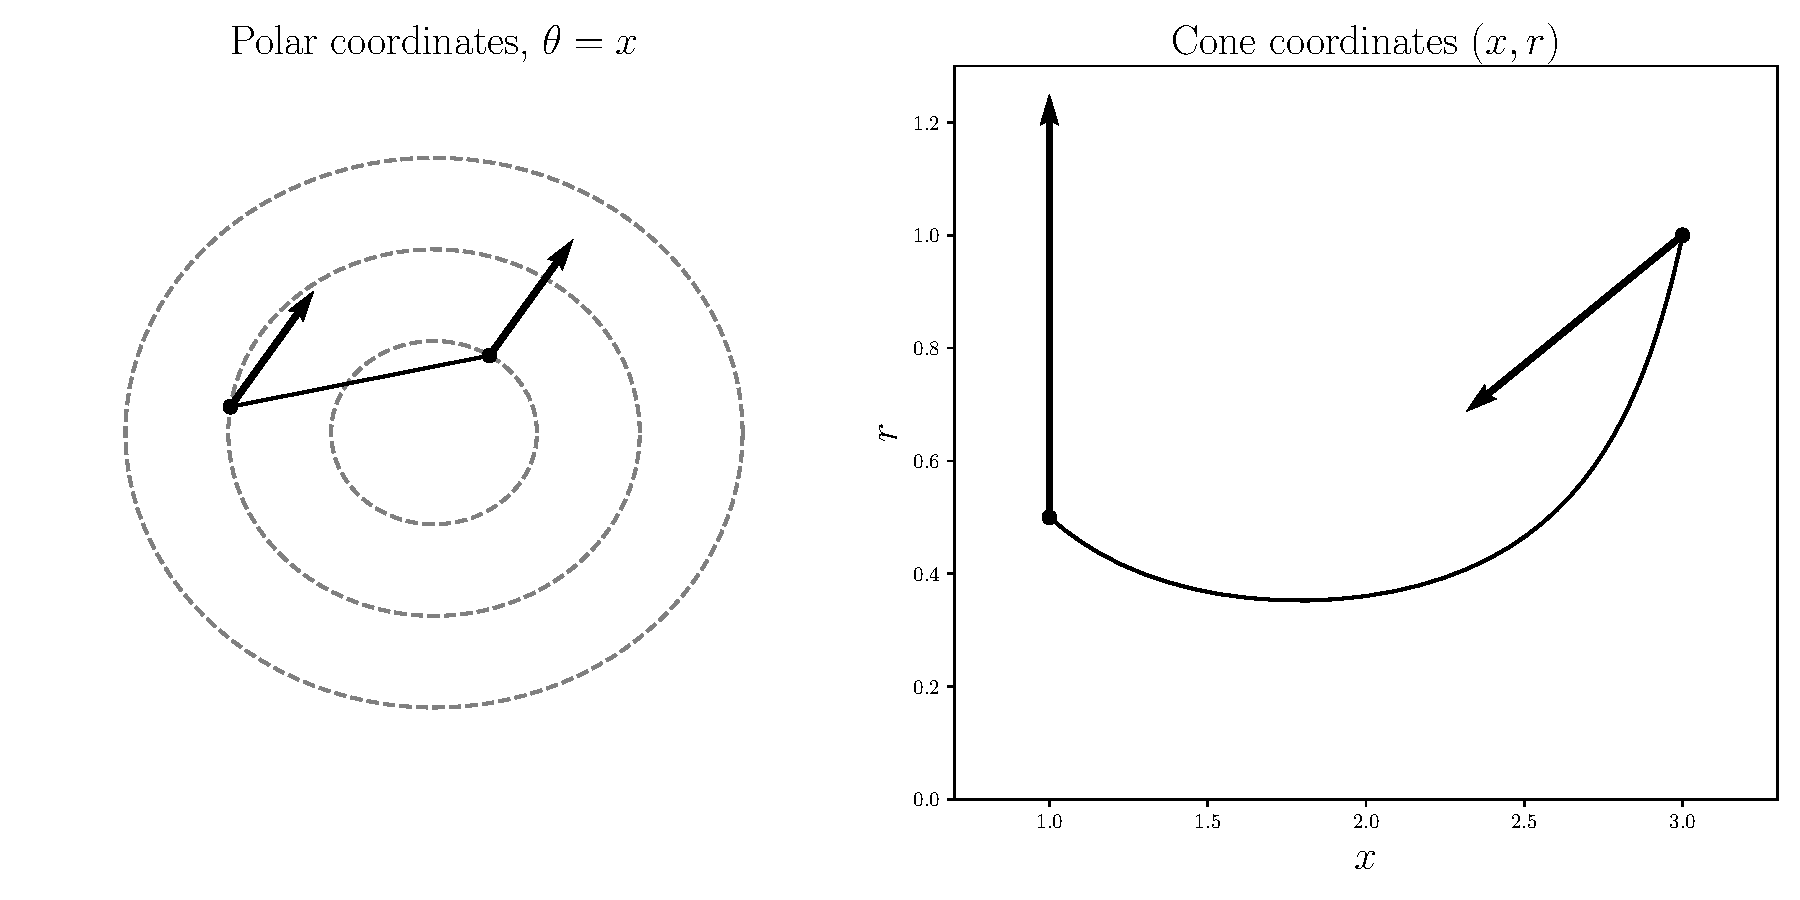
\includegraphics[width=\linewidth]{Figures/cone_parallel_transport_visualization.pdf}
    \caption{Visualization of geodesic parallel transport on $\mathfrak{C}_\Omega$ in polar coordinates (left) and cone coordinates (right). The visual consists of the parallel transport of $v = 0.75\partial_r$ from $(x_0, r_0) = (1.0, 0.5)$ to $(x_1, r_1) = (3.0, 1.0).$}
    \label{fig:cone_pt}
\end{figure}


\section{Proofs} \label{sec: proof of main results}

\subsection{Proof of \Cref{cone exponential and log map}.} \label{sec: proof of cone exponential and log map}

We desire a $z_1 \in \mathfrak{C}_\Omega$ such that $Z'(0^+; z_0, z_1)$, the right derivative at $0$, is equal to $(v_x, v_r).$ Letting $\theta = \|x_1 - x_0\|_2$, one can verify that 
\begin{align*}
    \rho'(s; z_0, z_1) = \frac{\sin^2(\theta)r_0r_1^2s}{\theta B(s)^{3/2}\sqrt{1 - \frac{A(s)^2}{B(s)}}}
\end{align*}
with 
\begin{equation*}
    A(s) = r_1s\cos(\theta) + r_0(1-s) \qquad B(s) = r_1^2s^2 + 2s(1-s)r_0r_1\cos(\theta) + r_0^2(1-s)^2.
\end{equation*}
We can directly evaluate $\lim_{s \rightarrow 0^+}B(s) = r_0^2$. For the radical,
\begin{align*}
    1 - \frac{A(s)^2}{B(s)} = \frac{\left(\frac{r_1s}{r_0(1-s)}\right)^2\sin^2(\theta)}{1 + 2\frac{r_1s}{r_0(1-s)}\cos(\theta) + \left(\frac{r_1s}{r_0(1-s)}\right)^2} = \left(\frac{r_1s}{r_0(1-s)}\right)^2\sin^2(\theta)\left(1 + u - u^2 + O(u^3)\right)
\end{align*}
where $u = 2\frac{r_1s}{r_0(1-s)}\cos(\theta) + \left(\frac{r_1s}{r_0(1-s)}\right)^2$. Plugging back in and canceling terms yields
\begin{align*}
    \lim_{s \rightarrow 0^+}\rho'(s; z_0, z_1) = \lim_{s\rightarrow 0^+}\left(\frac{\sin(\theta)r_1r_0^2(1-s)}{\theta B(s)^{3/2}\sqrt{1  + u - u^2 + O(u^3)}}\right) = \frac{\sin(\theta)r_1}{\theta r_0}
\end{align*}
since $\lim_{s \rightarrow 0^+}u = 0$, which implies $X'(0^+; z_0, z_1) = \frac{\sin(\theta)r_1(x_1 - x_0)}{\theta r_0}$. One can also easily verify that $R(0^+; z_0, z_1) = r_1\cos(\theta) - r_0$. Now we have a system of equations 
\begin{equation*}
    v_x = \frac{\sin(\|x_1 - x_0\|_2)r_1(x_1 - x_0)}{\|x_1 - x_0\|_2 r_0} \quad \text{and} \quad  v_r = r_1\cos(\|x_1 - x_0\|_2) - r_0
\end{equation*}
for which we know $(x_0, r_0)$ and we want to solve for $(x_1, r_1)$. One can verify that the solution is $r_1 = \sqrt{\|v_x\|_2^2r_0 + (v_r+r_0)^2}$ and $x_1 = x_0 + \theta\frac{v_x}{\|v_x\|_2}$ with $\theta = \operatorname{atan2}(r_0\|v_x\|_2, v_r + r_0) \in [0, \pi)$. This completes the exponential map. The logarithmic map is given by
$\log^{\mathfrak{C}}_{z_1}(z_0) = Z'(0^+; z_0, z_1)$, the expressions for which we have already derived in computing the exponential map.
\qed{}

\subsection{Proof of \Cref{radial update}} \label{sec: proof of radial update}
\begin{proof}
    By \Cref{lifting by characteristics one}, we have that
    \begin{align*}
    r_{i+1}^2 &= \frac{d\mu_{i+1}}{d\eta_{i+1}} = \frac{d(u_{i+1}(T_i)_\#\sigma_i)}{d((T_{i}\circ \cdots \circ T_1)_\#\mu_0)} = \frac{d(u_{i+1}(T_i)_\#\sigma_i)}{d((T_{i}\circ X_i)_\#\mu_0)} = \frac{d(u_{i+1}(T_i)_\#\sigma_i)}{d((T_{i})_\#\eta_i)}.
    \end{align*}
    Since the flow is bijective, we have
    \begin{align*}
        r_{i+1}^2 = u_{i+1}\frac{d\sigma_i}{d\eta_i} \circ T_i^{-1} = u_{i+1}\left(\frac{d\sigma_i}{d\mu_i}\frac{d\mu_i}{d\eta_i}\right)\circ T_{i}^{-1}.
    \end{align*}
    Since $\mu_i = u_i \sigma_i$, we have
    \begin{align*}
        r_{i+1}^2(x) = u_{i+1}(x)\left(\frac{r_i^2(T_i^{-1}(x))}{u_i(T_i^{-1}(x))}\right) \quad \text{and thus} \quad \frac{r_{i+1}^2(x)}{r_i^2(T_i^{-1}(x))} = \frac{u_{i+1}(x)}{u_i(T_i^{-1}(x))}.
    \end{align*}
    Applying the change of variables $y = T_i^{-1}(x)$ and taking the square root yields
    \[\frac{r_i(T_i(y))}{r_i(y)} = \sqrt{\frac{u_{i+1}(T_i(y))}{u_i(y)}}\]
    which completes the proof.
\end{proof}



\subsection{Proof of \Cref{isometry}.} \label{sec: proof of isometry}
We will start by showing that 
\[\mathcal{L}_{\mathfrak{B}\lambda, \lambda}: L^2(\mathfrak{B}\lambda; \Omega) \times L^2(\mathfrak{B}\lambda) \rightarrow L^2(\lambda; \mathfrak{C}_\Omega) \quad \text{given by} \quad \mathcal{L}_{\mu, \lambda}[(v, \beta)](x,r) = (v(x), 2\beta(x)r)\]
is an isometry. Let $s_1 = (v_1, \beta_1)$ and $s_2 = (v_2, \beta_2)$ be elements of $L^2(\mathfrak{B}\lambda; \Omega) \times L^2(\mathfrak{B}\lambda)$. Their inner product in the domain Hilbert space is given by 
\[\langle s_1, s_2\rangle_{\mathfrak{B}\lambda} = \int_{\Omega}\left( \langle v_1(x), v_2(x)\rangle + 4\beta_1(x)\beta_2(x)\right)d\mathfrak{B}\lambda(x) \]
where the inner product $\langle\cdot, \cdot\rangle$ is the standard Euclidean inner product on $\mathbb{R}^d$. For the lifted field, the inner product in the image is given by
\begin{align*}\langle \mathcal{L}[s_1], \mathcal{L}[s_2]\rangle_{\lambda} = \int_{\mathfrak{C}_\Omega} \langle \mathcal{L}[s_1], \mathcal{L}[s_2]\rangle_{\mathfrak{C}} d\lambda &= \int_{\mathfrak{C}_\Omega}r^2\left(4\beta_1(x)\beta_2(x) + \langle v_1(x), v_2(x) \rangle\right)d\lambda(x,r) \\
&= \int_\Omega \left(4\beta_1(x)\beta_2(x) + \langle v_1(x), v_2(x) \rangle\right)d\mathfrak{B}\lambda(x)
\end{align*}
by \Cref{eq: measure projection}. Thus, $\langle \mathcal{L}[s_1], \mathcal{L}[s_2]\rangle_{\lambda} = \langle s_1, s_2\rangle_{\mathfrak{B}\lambda}$ proving (a). Now we will prove (b). Let $u, v \in L^2(\lambda; \mathfrak{C}_\Omega)$ where $u = a + b\partial_r$ and $v = c + d\partial_r$. Their inner product in the domain Hilbert space is given by
\begin{align*}
    \langle u, v\rangle_{\lambda} &= \int_{\mathfrak{C}} \langle u, v \rangle_{\mathfrak{C}}\,d\lambda = \int_{\mathfrak{C}} \left(b(x,r)d(x,r) + r^2\langle a(x,r), c(x,r)\rangle \right)\,d\lambda(x,r)
\end{align*}
where the inner product on the right is the standard Euclidean inner product on $\mathbb{R}^d$. By the hypothesis, the radial law of $\lambda$ is deterministic given $x$. Thus, the projections of $u$ and $v$ are given by $\mathcal{P}_{\lambda}[u](x) = (a(x,r(x)), b(x,r(x))/2r(x))$ and $\mathcal{P}_{\lambda}[v](x) = (c(x,r(x)), d(x,r(x))/2r(x))$ and their inner product is
\begin{align*}
    \langle \mathcal{P}_{\lambda}[u], \mathcal{P}_{\lambda}[v]\rangle_{\mathfrak{B}\lambda} &= \int_{\Omega} \left(\frac{4b(x, r(x))d(x, r(x))}{4r^2(x)} +  \langle a(x, r(x)), c(x,r(x)\rangle\right)d\mathfrak{B\lambda}(x) \\
    &= \int_{\Omega}\left(\frac{b(x, r(x))d(x, r(x))}{r^2(x)} +  \langle a(x, r(x)), c(x,r(x)\rangle\right)d\mathfrak{B\lambda}(x) \\
    &= \int_{\mathfrak{C}_\Omega}\left(b(x, r(x))d(x, r(x)) +  r^2(x)\langle a(x, r(x)), c(x,r(x)\rangle\right)d\lambda(x, r(x))
\end{align*}
which is equivalent to $\langle u, v \rangle_\lambda$. \qed{}

\subsection{Proof of \Cref{lifting by characteristics one}} \label{sec: proof of lifting by characteristics one}

\begin{proof}
    Let $\nu_t = r_t^2 \eta_t$. Since $\eta_t = (X_t)_\# \mu_0$, for every bounded test function $\varphi$,
    \[\int_\Omega \varphi(x) \, d\eta_t(x) = \int_{\Omega} \varphi(X_t(x)) \, d\mu_0(x).\]
    By the definition of $r_t$ along the characteristic flow $X_t$, we have
    \begin{multline*}
    \int_\Omega \varphi(x) \, d\nu_t(x) = \int_\Omega \varphi(x) r_t(x)^2 \, d\eta_t(x) = \int_{\Omega} \varphi(X_t(x)) r_t(X_t(x))^2 \, d\eta_0(x)\\
    = \int_{\Omega} \varphi(X_t(x)) \exp\left(4\int_0^t \beta_s(X_s(x))\, ds\right) \, d\mu_0(x) \end{multline*}
    and thus
    \[\int_\Omega \varphi(y) \, d\nu_t(y) =\int_{\Omega} \varphi(X_t(x)) \exp\left(4\int_0^t \beta_s(X_s(x))\, ds\right) \, d\mu_0(x).\]
    Differentiating in time yields
    \begin{align*}
        \frac{d}{dt}\int_\Omega \varphi \, d\nu_t = \int_\Omega (\nabla \varphi \cdot v_t + 4\beta_t \varphi) \, d\nu_t
    \end{align*}
    which implies that $\nu_t = r_t^2 \eta_t$ solves the continuity-reaction equation weakly with initial condition $\nu_0 = \mu_0$. The assumption of the uniqueness guarantees that $\nu_t = \mu_t$. To verify the lifting property, observe that for any continuous $\phi$
    \begin{align*}
        \int_\Omega \phi \,d\mathfrak{B}\lambda_t = \int_{\mathfrak{C}_\Omega} r^2 \phi \, d\lambda = \int_\Omega r_t^2(x)\phi(x) \, d\eta_t(x) = \int_\Omega \phi \,d\mu_t
    \end{align*}
    which completes the proof.
\end{proof}

\subsection{Proof of \Cref{lifting by characteristics two}} \label{sec: proof of lifting by characteristics two}

\begin{proof}
    Recall, $\lambda_t = (x \mapsto (x, r_t(x))_\# \eta_t$. By construction, the conditional radial law of $\lambda_t$ is deterministic. By \Cref{isometry}, we know that $\mathcal{L}_{\mu_t, \lambda_t}$ and $\mathcal{P}_{\lambda_t}$ are isometric inverses from $T_{\mu_t}\mathfrak{M}_+(\Omega)$ to $T_{\lambda_t}\mathcal{P}_2(\mathfrak{C}_\Omega)$. Now we will show that the lifted tangent field $V_t = \mathcal{L}_{\mu_t, \lambda_t}(v_t, \beta_t)$ and the lifted curve of measures $\lambda_t$ satisfy the continuity equation on $\mathfrak{C}_\Omega$ weakly. Let $\Phi \in C^\infty_c(\mathfrak{C}_\Omega)$, and observe that  
    \begin{align*}
        \int_{\mathfrak{C}_\Omega}\Phi(x,r) \, d\lambda_t(x,r) &= \int_{\mathfrak{C}_\Omega} \Phi(x, r_t(x))\, d\eta_t = \int_{\mathfrak{C}_\Omega} \Phi\left(X_t(x), r_t\left(X_t(x)\right)\right) \, d\eta_0.
    \end{align*}
    Define $F_t(x) \triangleq (X_t(x), r_t(X_t(x))) \in \mathfrak{C}_\Omega$. Differentiating the leftmost and rightmost expressions yields
    \begin{align*}
        \frac{d}{dt}\int_{\mathfrak{C}_\Omega}\Phi(x,r) \, d\lambda_t(x,r) &=  \int_{\mathfrak{C}_\Omega} \frac{d}{dt}\Phi\left(X_t, r_t\left(X_t\right)\right) \, d\eta_0 \\
        &= \int_{\mathfrak{C}_\Omega} \left[\nabla_x\Phi(x,r) \partial_tX_t + \partial_r \Phi(x,r)\partial_tr_t(X_t)\right]\Big|_{(x,r) = F_t(x)} d\eta_0.
    \end{align*}
    Note that $V_t$ can be equivalently expressed by $(\partial_t X_t(x), \partial_t [r_t(X_t)])$ since $\partial_t[r_t(X_t)] = 2r_t(X_t)\beta_t(X_t)$. Thus, the righthand side of the panel above is 
    \begin{align*}
        \int_{\mathfrak{C}_\Omega} \left\langle \nabla_{\mathfrak{C}}\Phi(F_t), V_t(F_t)\right\rangle_{\mathfrak{C}} \,d\eta_0 = \int_{\mathfrak{C}_\Omega} \left\langle \nabla_{\mathfrak{C}}\Phi(x, r_t(x)), V_t(x, r_t(x))\right\rangle_{\mathfrak{C}} \,d\eta_t(x)
        = \int_{\mathfrak{C}_\Omega}\langle \nabla_{\mathfrak{C}}\Phi, V_t\rangle_{\mathfrak{C}} \, d\lambda_t.
    \end{align*}
    Thus,
    \[\frac{d}{dt}\int_{\mathfrak{C}_\Omega}\Phi(x,r) \, d\lambda_t(x,r) = \int_{\mathfrak{C}_\Omega}\langle \nabla_{\mathfrak{C}}\Phi, V_t\rangle_{\mathfrak{C}} \, d\lambda_t\]
    which is exactly the weak form of the continuity equation on $\mathfrak{C}_\Omega$. To show that the lift is optimal, consider the following. Since $(\lambda_t, V_t)$ satisfy the continuity equation, by the Benamou-Brenier formula we know that 
    \[W_\mathfrak{C}(\lambda_0, \lambda_1)^2 \leq \int_0^1\|V_t\|_{L^2(\lambda_t)}^2 \, dt.\]
    By the isometry of $\mathcal{P}_{\lambda_t}$, we have
    \begin{align*}
        W_{\mathfrak{C}}(\lambda_0, \lambda_1)^2 \leq \int_0^1 \|(v_t, \beta_t)\|_{\mu_t}^2 \, dt &= \HK(\mu_0, \mu_1)^2
    \end{align*}
    since $\mu_t$ is a geodesic and $(v_t, \beta_t, \mu_t)$ solve the continuity-reaction equation. For the reverse inequality, the characterization given in \Cref{eq: cone wasserstein and hk equivalence} indicates that $W_\mathfrak{C}(\lambda_0, \lambda_1)^2 \geq \HK(\mu_0, \mu_1)^2$. Thus, $W_\mathfrak{C}(\lambda_0, \lambda_1) = \HK(\mu_0, \mu_1)$ and the lifts $\lambda_0, \lambda_1$ are optimal. It also follows that $\lambda_t$ is a $W_\mathfrak{C}$ geodesic.
\end{proof}

\subsection{Proof of \Cref{uniformly bounded lifts}} \label{sec: proof of uniformly bounded lifts}

\begin{proof}
    Recall that $r_t$ along the characteristic flow $X_t$ is given by
    \[r_t(X_t(x)) = \exp\left(2\int_0^t \beta_s(X_s(x))\, ds\right).\]
    Thus, since $\beta_t$ satisfies
    $\operatorname{essinf}_{\mu_t} \beta_t \geq \beta_{\min}$ and $\esssup_{\mu_t}\beta_t \leq \beta_{\max}$
    for some $\beta_{\min} > -\infty, \beta_{\max} < \infty$ independent of $t$, then 
    \[  \beta_{\max}t\geq \int_0^t\beta_s(X_s(x)) \, ds \geq \beta_{\min}t\]
    and $r_{\max}\triangleq \exp(2\max\{\beta_{\max}, 0\})\geq r_t(X_t(x)) \geq \exp\left(2 \min\{\beta_{\min}, 0\}\right) \triangleq r_{\min}$.
\end{proof}

\subsection{Proof of \Cref{uniformly regular lifts}} \label{sec: proof of uniformly regular lifts}

\begin{proof}
    Recall the definition $V_t(x,r) = (v_t(x), 2\beta_t(x)r)$. We will start by proving the integrability result. By the isometry of the lifting procedure (\Cref{lifting by characteristics two}), we have
    \begin{align*}
        \int_0^1 \|V_t\|_{L^2(\lambda_t)}^2 \, dt &= \int_0^1 \int_{\Omega} \|(v_t, \beta_t)\|_{L^2(\mu_t)}^2 \, dt \\
        &= \int_0^1 \|v_t\|_{L^2(\mu_t)}^2\, dt + 4\int_0^1|\beta_t|^2_{L^2(\mu_t)}\, dt \\
        &< \infty 
    \end{align*}
    by \Cref{interpolant regularity}. For the second result, note that we can bound the spatial Lipschitz constant of a vector field on a manifold using the covariant derivative \citet[Proposition 10.46]{boumal2023introduction}. In particular, $V_t$ is $L$-Lipschitz continuous if and only if $\|\nabla^{\mathfrak{C}}_UV_t\|_{\mathfrak{C}} \leq L\|U\|_{\mathfrak{C}}$ for all $U\in T\mathfrak{C}_\Omega$. Let $U = a + b\partial_r \in T\mathfrak{C}_\Omega$ be a tangent field and write $V_t = c_t + d_t \partial_r$ where $c_t(x,r) = v_t(x)$ and $d_t(x,r) = 2\beta_t(x)r$. The covariant derivative of $V_t$ in the direction $U$ is given by 
    \begin{align*}
        \nabla^{\mathfrak{C}}_{U}V_t &= \nabla_a^{\mathfrak{C}}V_t + b \nabla ^{\mathfrak{C}}_{\partial_r}V_t \\
        &= \nabla_a^{\mathfrak{C}}c_t + \nabla_a^{\mathfrak{C}}(d_t\partial_r) + b\nabla ^{\mathfrak{C}}_{\partial_r}c_t + b\nabla_{\partial_r}^{\mathfrak{C}}(d_t\partial_r).
    \end{align*}
    Now we will apply \Cref{corollary: connection on cone}. The first term is
    \begin{align*}
        \nabla_a^{\mathfrak{C}}c_t &= \nabla v_t^\top a - r\langle v_t, a\rangle \partial_r.
    \end{align*}
    The second term can be simplified by applying the Leibniz rule, which gives
    \begin{align*}
        \nabla _a^\mathfrak{C}(d_t\partial_r) &= a(d_t)\partial_r + d_t \nabla_a^\mathfrak{C}\partial_r \\
        &= 2ra(\beta_t) \partial_r + 2\beta_ta.
    \end{align*}
    For the third term, we have $b\nabla_{\partial_r}^\mathfrak{C}c_t = bv_t/r$, and for the fourth term we have
    \begin{align*}
        b\nabla_{\partial_r}^{\mathfrak{C}}d_t\partial_r &= b\left(\partial_r(d_t) + d_t\nabla^\mathfrak{C}_{\partial_r}\partial_r\right)\partial_r \\
        &= 2b \beta_t\partial_r.
    \end{align*}
    Thus,
    \[\nabla^{\mathfrak{C}}_{U}V_t = \nabla v_t^\top a + 2 \beta_t a+ \frac{bv_t}{r} + \left(2ra(\beta_t) + 2b\beta_t - r\langle v_t, a\rangle\right)\partial_r.\]
    Taking the norm and applying the triangle inequality yields
    \begin{align}
        \left\| \nabla^\mathfrak{C}_U V_t\right\|_{\mathfrak{C}_\Omega} &\le  r\left\|\nabla v_t \right\|_{\operatorname{op}}\|a\|_2 + 2r|\beta_t|\|a\|_2 + |b|\|v_t\|_2 + 2r|a(\beta_t)| + 2|b||\beta_t| + r\|v_t\|_2\|a\|_2. \label{cov deriv upper bound}
    \end{align}
    We'll continue to upper bound these terms until we arrive at something that is a constant multiple of $\|U\|_\mathfrak{C}$. Since $a$ has no radial component, we have
    \begin{align*}
        |a(\beta_t)| &= |\langle \operatorname{grad}^\mathfrak{C}\beta_t, a \rangle_{\mathfrak{C}}| = r^2|\langle r^{-2}\nabla \beta_t, a\rangle | \leq \|\nabla \beta_t\|_2\|a\|_2.
    \end{align*}
    Also observe that we have the following bounds $r\|a\|_2 \leq \|U\|_{\mathfrak{C}}$ and $|b| \leq \|U\|_{\mathfrak{C}}$; when applied to \cref{cov deriv upper bound} this yields
    \begin{align*}
        \left\| \nabla^\mathfrak{C}_U V_t\right\|_{\mathfrak{C}_\Omega} &\le  \left(\left\|\nabla v_t \right\|_{\operatorname{op}} + 2\|\nabla \beta_t\|_2 + 2\|v_t\|_2  + 4|\beta_t|\right)\|U\|_{\mathfrak{C}}
    \end{align*}
    and taking the supremum over $(x,r)$ yields
    \begin{align*}
        \sup_{(x,r)\in \mathfrak{C}_\Omega}\left\| \nabla^\mathfrak{C}_U V_t\right\|_{\mathfrak{C}_\Omega} &\le  \left(\left\|\nabla v_t \right\|_{L^\infty} + 2\|\nabla \beta_t\|_{L^\infty} + 2\|v_t\|_{L^\infty}  + 4\|\beta_t\|_{L^\infty}\right)\|U\|_{\mathfrak{C}}.
    \end{align*}
    The properties of the measures in the admissible class (\Cref{admissible class}) guarantee that the quantity in the parentheses is bounded by some $L < \infty$ for all $t$, completing the proof.
\end{proof}

\subsection{Proof of \Cref{cone ambient manifold}} \label{sec: proof of cone ambient manifold}
\begin{proof}
    We will proceed with a proof by construction. By \Cref{uniformly bounded lifts} there exist constants $r_{\min}, r_{\max} > 0$ such that $\operatorname{supp} \lambda_t \subset \Gamma \times[r_{\min}, r_{\max}] \triangleq K$ for all $t \in [0,1]$. Let $U$ be an open neighborhood of $\Gamma$ with $\Gamma \Subset U \Subset \Omega^\circ$ and define 
    \[\mathcal{U} \triangleq U \times (r_{\min}/2,2 r_{\max}) \subset \mathfrak{C}_\Omega.\]
    Since $\mathcal{U}$ is contained in the smooth part of the cone and stays uniformly bounded away from the apex, it is a smooth, open (and thus boundaryless) manifold endowed with the cone metric $g_\mathfrak{C}$. Now, choose an open set $W$ such that $K \Subset W \Subset \mathcal U$. Since $\mathcal U$ is a smooth manifold without boundary, there exists a smooth complete
    Riemannian metric $h$ on $\mathcal U$ \citep{nomizu1961existence}. Let $\chi \in C_c^\infty(\mathcal U)$ satisfy
    \[
    0 \leq \chi \leq 1, \qquad \chi \equiv 1 \text{ on } W.
    \]
    Define the augmented metric tensor
    \[
    \widetilde g_{\mathfrak C} \triangleq \chi g_{\mathfrak C} + (1-\chi)h.
    \]
    Since $g_{\mathfrak C}$ and $h$ are smooth positive-definite bilinear forms, so is
    $\widetilde g_{\mathfrak C}$; hence $\widetilde g_{\mathfrak C}$ is a smooth Riemannian metric
    on $\mathcal U$. Moreover, $\widetilde g_\mathfrak{C}$ coincides with $g_\mathfrak{C}$ on  a neighborhood of
    $\bigcup_{t\in[0,1]}\operatorname{supp}\lambda_t \subset K$. We next show that $\widetilde g_{\mathfrak C}$ is complete. On the compact set
    $\operatorname{supp}\chi$, the smooth metrics $g_{\mathfrak C}$ and $h$ are uniformly equivalent (due to positive definiteness),
    so there exists $c>0$ such that
    $g_{\mathfrak C} \geq c h$ on $\operatorname{supp}\chi.$ Therefore, on $\operatorname{supp}\chi$,
    \[
    \widetilde g_{\mathfrak C}
    = \chi g_{\mathfrak C} + (1-\chi)h
    \geq \chi c\, h + (1-\chi)h
    \geq \min\{1,c\}\, h.
    \]
    Outside $\operatorname{supp}\chi$ we have $\widetilde g_{\mathfrak C}=h$. Hence, we have the global bound $\widetilde g_{\mathfrak C} \geq c_0 h$ for some constant $c_0 > 0$. This bound in combination with the completeness of $h$ guarantees that $\tilde g_\mathfrak{C}$ is complete. This proves (1) and (2). It remains to verify (3). By construction,
    \[
    \operatorname{supp}\lambda_t \subset K \Subset W
    \qquad \forall t\in[0,1],
    \]
    and $\widetilde g_{\mathfrak C}=g_{\mathfrak C}$ on $W$. Hence all geometric quantities computed
    along the lifted curve $(\lambda_t,V_t)$ agree whether they are evaluated using $g_{\mathfrak C}$
    or $\widetilde g_{\mathfrak C}$. In particular, by \Cref{uniformly regular lifts},
    $(\lambda_t)$ satisfies the continuity equation on $\mathcal U$ with velocity field $V_t$, and
    \[
    \int_0^1 \|V_t\|_{L^2(\lambda_t)}\,dt < \infty,
    \qquad
    \sup_{t \in [0,1]} \operatorname{Lip}^{\widetilde g_{\mathfrak C}}(V_t) < \infty,
    \]
    since the corresponding Lipschitz bounds coincide on $W$, which contains the supports of
    $\lambda_t$. Thus $(\lambda_t)$ is a regular curve in
    $\mathcal P_2(\mathcal U,\widetilde g_{\mathfrak C})$. Finally, since $(\mathcal U,\widetilde g_{\mathfrak C})$ is a smooth and complete manifold without
    boundary, Gigli's parallel transport theory applies to $(\lambda_t)$. Moreover, because
    $\widetilde g_{\mathfrak C}$ agrees with $g_{\mathfrak C}$ on a neighborhood of the lifted curve,
    all tangent spaces, orthogonal projections, and partition-based transport operators arising in
    Gigli's construction coincide with those obtained from the original cone geometry along
    $(\lambda_t)$. Therefore the resulting parallel transport objects depend only on the original
    cone geometry along the lifted curve.
\end{proof}

{\bibliography{main.bib}}

\end{document}
